%%%%%%%%%%%%%%%%%%%%%%%%%%%%%%%%%%%%%%%%%%%%%%%%%%%%%%%%%%%%%%%%%%%%%%%
%% Zusammenfassung und Ausblick
\section{Entwicklung}
\label{sec:entwicklung}
Dieses Kapitel befasst sich mit einzelnen Aspekten der Entwicklung. Nach der Auflistung der Nicht-funktionalen Anforderungen, sowie der Funktionen, werden grundlegende Konzepte und Architekturen vorgestellt. Dabei werden erste Sensoren, Aktoren und bestehende Software Bibliotheken getestet und für eine Anschlussverwendung bewertet. Die weiteren benötigten Softwarepaket werden im nachfolgenden Kapitel Implementierung TODO umgesetzt.

\subsection{Nicht-Funktionale Anforderungen}
\label{sec:dev-nichtfunk}

Die nicht-funktionalen Anforderungen beschreiben Qualitätsmerkmale des MRS. Diese sind in verschiedene Kategorien gruppiert und haben Auswirkungen auf die Funktionalität und die Architektur. Im Folgenden werden nur die für diese Arbeit relevanten Kategorien erläutert und in Bezug gebracht.

\subsubsection{Sicherheit - Safety}

Im englischen wird der Begriff Sicherheit in die Terme \textit{Security} und \textit{Safety} unterteilt. Ersteres beschäftigt sich unter anderem mit der Verschlüsselung von Daten. Der Begriff \textit{Safety} bezieht sich auf die Anwendersicherheit, zum Beispiel ob dieser durch das System Verletzungen erleiden kann oder ob sich das System selbst oder die Umwelt beschädigt. Da die Roboter in dieser Arbeit nicht, wie Industrieroboter, durch Gitterzäune gesichert sind wird eine Lichtwarnanlage installiert. Diese arbeitet ähnlich einer Ampel. Befindet sich das System in einer sicheren Stellung, in der es sich nicht bewegt, leuchtet die Lichtanlage in grün. Wird eine Bewegung geplant oder ist das System vor einer Bewegung blinkt die Lichtanlage fünf Sekunden gelb. Innerhalb dieses Intervalls bewegt sich das System nicht. Auf das Blinken folgt ein rotes Leuchten der Lichtanlage. In dieser Zeit führen die Roboter ihre Aktionen aus. Während dieser Aktionen nutzt das Robotersystem die Sensoren und berechnet kollisionsfreie Pfade um nicht mit sich selbst oder der Umwelt zu kollidieren. Objekte, die sich erst zur Laufzeit auf dem Pfad befinden, werden in dieser Arbeit noch nicht beachtet und können so zur Kollision führen. Um bei Bewegungen der mobilen Plattform oder zwischen zwei Tasks der Arme die Sicherheit dieser zu sicheren existieren die beiden Posen \textit{Candle} und \textit{Fold}. Die erste Pose streckt den Arm senkrecht in die Höhe und ermöglicht so kollisionsfreie Pfade in die meisten anderen Posen. In der zweiten Pose befinden sich alle Gelenke in ihrer minimalen Konfiguration. Sollte dem Roboter der Strom fehlen, bedingt durch einen Stromausfall oder leere Batterien, fällt der Roboterarm in sich zusammen, da die Gelenkmotoren die Position nicht mehr halten können. In der \textit{Fold}-Pose kann der Roboter nicht weiter in sich zusammenfallen, da alle Glieder aufeinander liegen. Deshalb sollten die Roboter diese Pose in längeren Inaktivitätsphasen einnehmen. Diese Aspekte werden während der Entwicklung der Funktionen berücksichtigt.

\subsubsection{Zuverlässigkeit}
Die Zuverlässigkeit des Systems beschreibt unter anderem das Systemverhalten bei einem Fehlerfall oder Teilsystemausfall. Das Robotersystem darf dabei nicht in einen unsicheren Zustand geraten. Da das Robotersystem auf ROS aufbaut werden einzelne Aktoren und Sensoren als ROS-Node betrieben. Jeder Node stellt dabei ein einzelnes Subsystem dar, welcher ausfallen kann. ROS ist so konzipiert, dass das ganze System nicht abstürzt, wenn ein einzelner Node ausfällt. Eine Schwachstelle bildet hierbei der ROS-Core. Dieser stellt den Mittelpunkt eines ROS-Systems dar. Fällt dieser aus bricht die Kommunikation zwischen den einzelnen Nodes zusammen. In diesem Fall müssen die Nodes in einen sicheren Fehlerzustand übergehen. Dies betrifft vor allem die Aktoren, besonders die Steuerungen der Roboter. 

Ein weiterer Aspekt der Zuverlässigkeit ist die Wiederherstellbarkeit. Dies betrifft ob und wie komplex ein bestimmter fehlerfreier Systemstatus wiederhergestellt werden kann. Da die Nodes einzelne Subsysteme sind, können diese nach einem Ausfall einfach wieder gestartet werden und der Systemstatus ist wiederhergestellt. Dies betrifft auch den ROS-Core. Wird dieser auf der selben Adresse (IP und Port) neu gestartet, nehmen alle Nodes die Kommunikation wieder auf. Diese beiden Aspekte werden vor allem bei der Entwicklung der Architektur für das MRS berücksichtigt. Dabei ist das zentrale Koordinierungs- und Konfigurations-System eine Komponente, die zu einem potenziellen Single-Point-of-Failure führen kann.


\subsubsection{Korrektheit}
Die Korrektheit lässt sich in dieser Entwicklung durch die Genauigkeit der Funktionen definieren. So dürfen die Positionen und Orientierungen der Arme und der mobilen Plattform nur um bestimmte Grenzen abweichen. Dabei gelten für die End-Effektor-Pose eine Distanzabweichung von maximal 5mm für jede Dimension und für die Orientierung eine Abweichung von maximal 1\textdegree pro Achse. Dies muss bei der Entwicklung der inversen Kinematik berücksichtigt werden. Für die mobile Plattform gelten andere maximale Abweichungen. Für die Distanzabweichungen sind das 5cm in X- und Y-Richtung. Für die Z-Dimension darf sie maximal 5mm sein. Für die Rotation gilt: Z-Achse 5\textdegree, X- und Y- Achse 1\textdegree.

\subsubsection{Leistung}
Die Leistung bezieht sich auf die Effizienz des MRS. Besonders der Zeit- und Energieaufwand sollen möglichst minimiert werden. Der Zeitaufwand bezieht sich dabei nicht auf die Performance-Optimierung der Algorithmen, sondern der Bewegungen und deren Abläufe. Dieser Aspekt muss bei der Entwicklung der Funktionen und der Implementierung berücksichtigt werden. Der Energieaufwand ist stark abhängig von den benutzten Aktoren und wird bei der Entwicklung der inversen Kinematik für die Arme und die Pfadbestimmung für die mobile Plattform in Betracht gezogen.

\subsubsection{Änderbarkeit}
Die Änderbarkeit besteht aus Sicht der Entwicklung aus mehreren Aspekten. Für diese Arbeit ist dabei die Erweiterbarkeit ein wichtiger Aspekt. Zum einen geht es um die Erweiterbarkeit des MRS um weitere Sensoren und Aktoren. Diese sollen möglichst einfach in das bestehende MRS eingebunden werden können ohne bestehende Subsysteme zu verändern. Zum anderen soll in der Weiterentwicklung dieses MRS weitere Konzepte eingebunden werden. So müssen für eine automatische Konfiguration und verteilte Koordinierung Schnittstellen in der Architektur entworfen werfen. Diese Schnittstellen sollen unter anderem eine Markt-basierte Konfiguration ermöglichen. Diese beiden Aspekte der Erweiterbarkeit müssen in der Entwicklung der Architektur und der Funktionen berücksichtigt werden. So sind grobe Kostenangaben für die Funktionen ein möglicher Ansatz für die Gebote am Markt.

\subsection{Funktionalitäten}
\label{sec:dev-funk}

In diesem Kapitel werden die Funktionen des Robotersystem aufgelistet. Das folgende Use-Case Diagramm \ref{fig:dev-usecase} stellt die groben Funktionsanforderungen an das Robotersystem dar.

\begin{figure}[H]
	\centering
	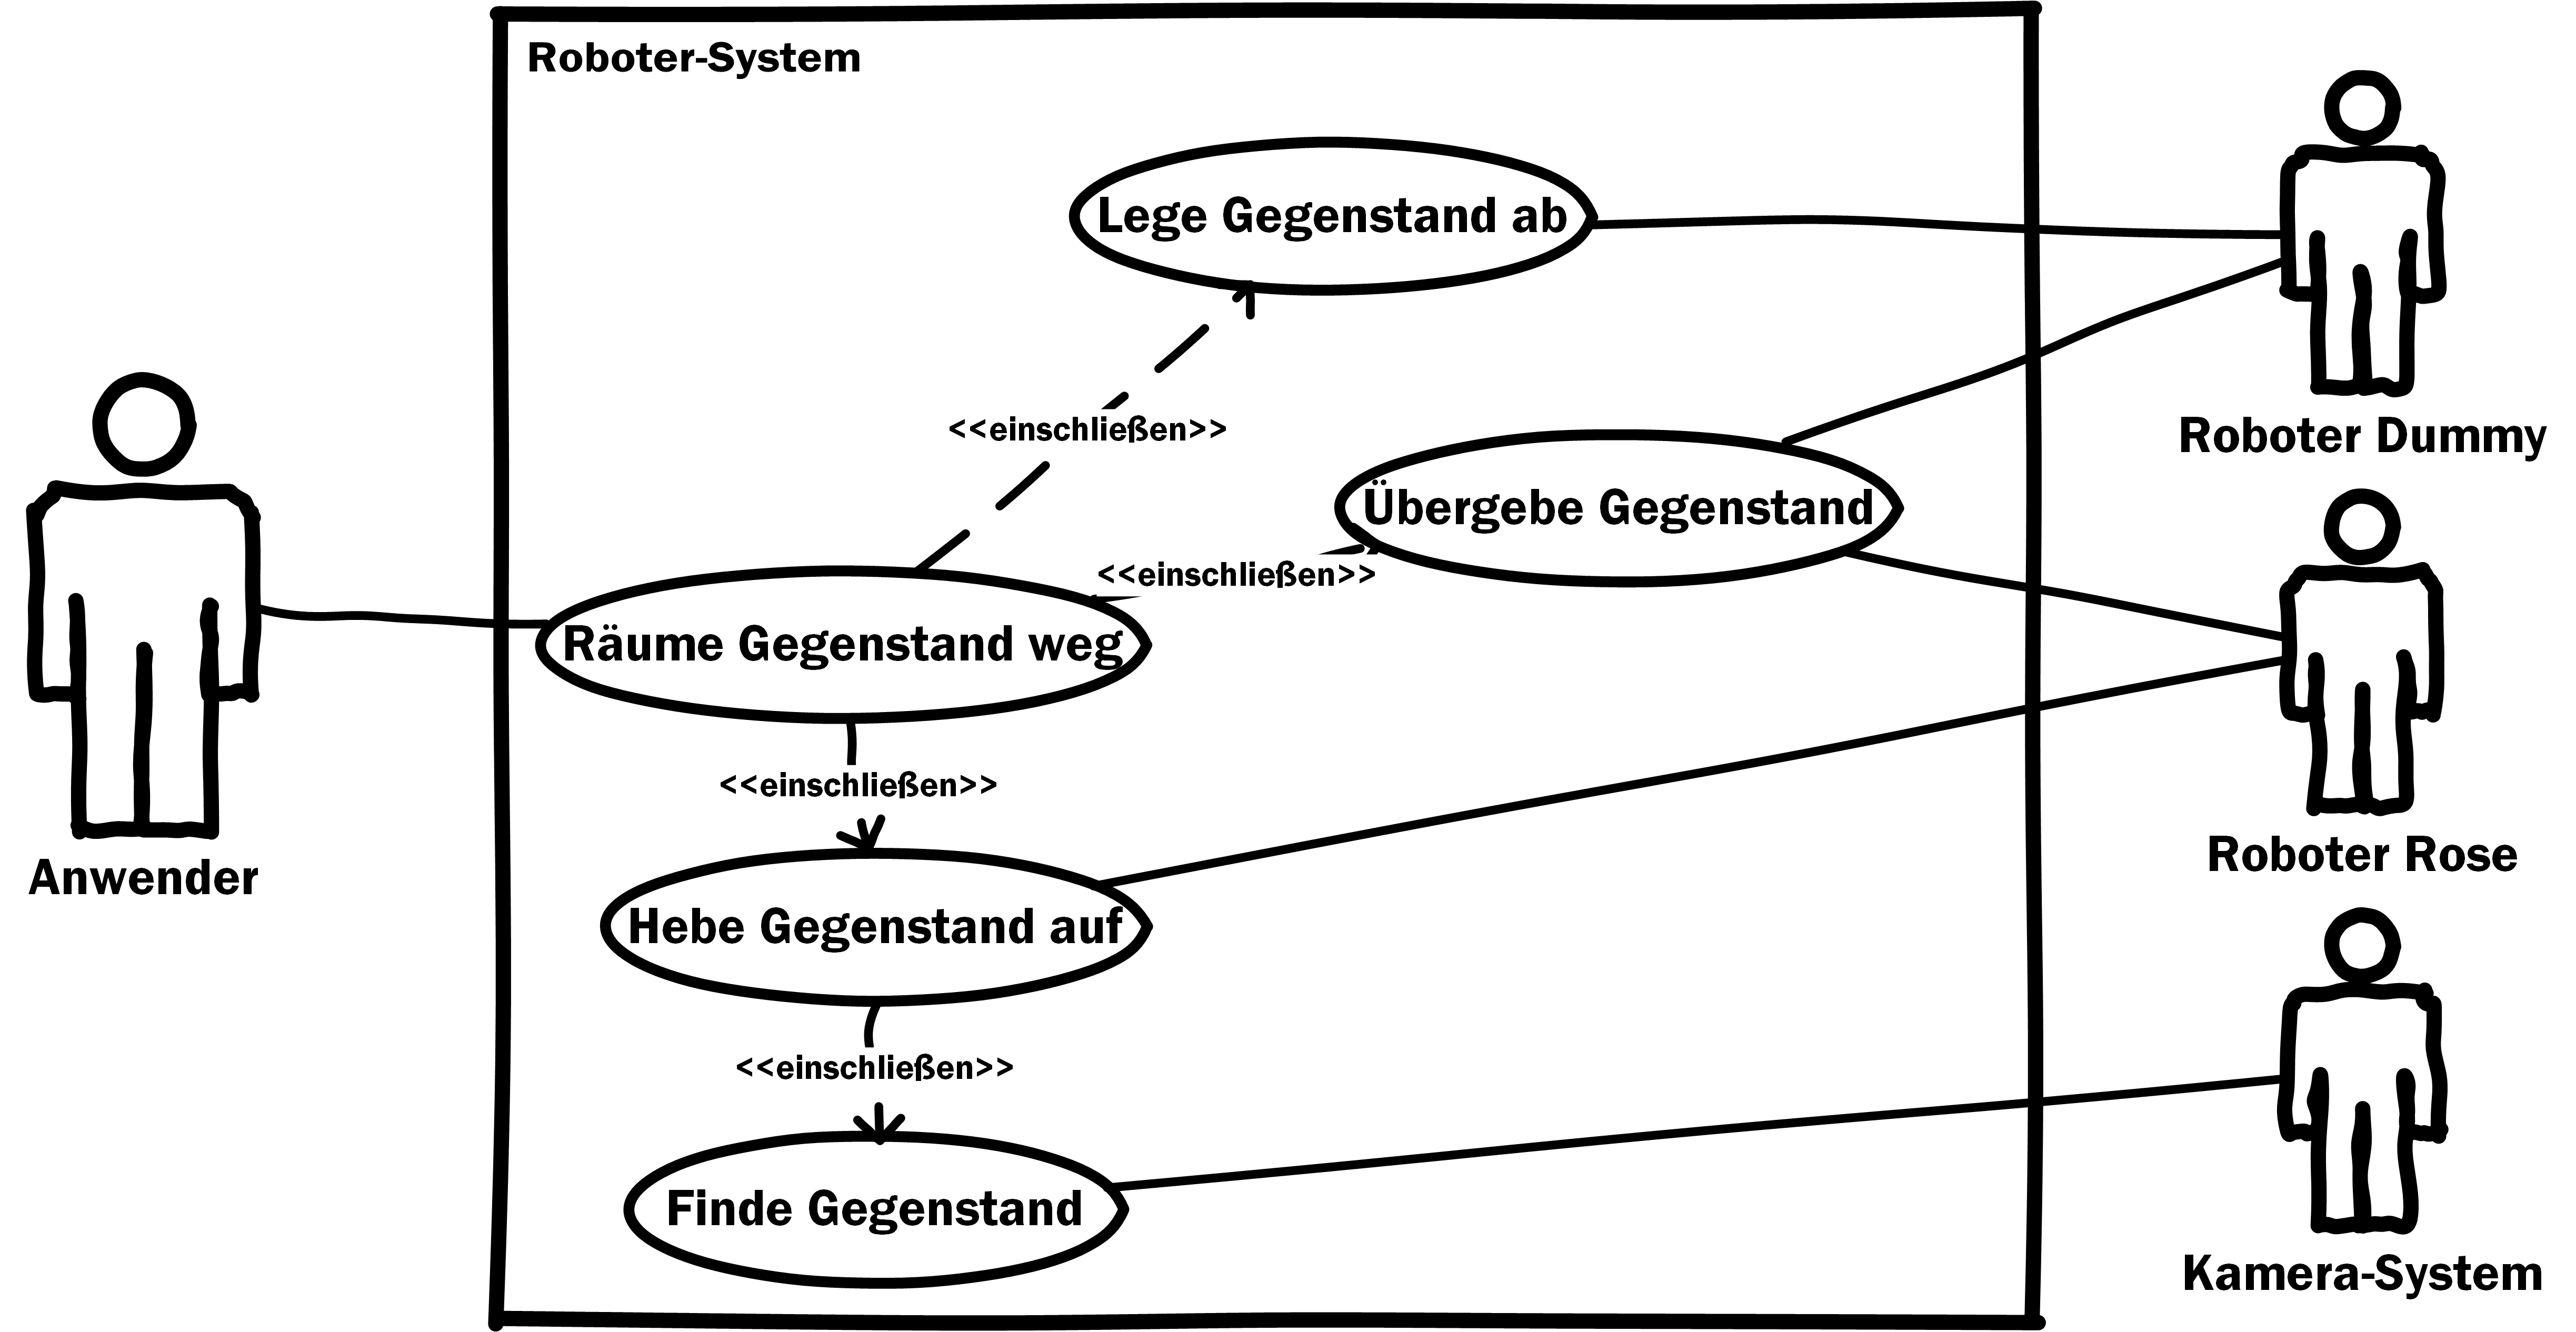
\includegraphics[scale=0.8]{fig/UseCase}   
	\caption[Use-Case Robotersystem]{Vereinfachtes Use-Case Diagramm zur groben Funktionsübersicht des Robotersystems}
	\label{fig:dev-usecase}
\end{figure}

Der Anwender gibt dem System die Anweisung einen Gegenstand wegzuräumen. Das Robotersystem gliedert die Anweisung in einzelne Tasks auf. Diese Tasks werden von den unterschiedlichen Akteuren mit ihren Funktionalitäten sequentiell oder parallel ausgeführt. In diesem konkreten Fall soll zunächst der Roboter Rose den entsprechenden Gegenstand aufheben. Dies erfordert zunächst eine Lokalisierung des Objektes die von einem Kamerasystem angefordert wird. Anschließend übergeben sich die Roboter Rose und Dummy den Gegenstand, bevor Dummy ihn anschließend an einer gewünschten Position ablegt. Diese sehr grobe Darstellung des Vorgangs beinhaltet die vier zentralen Funktionen, die das System umsetzen muss: Gegenstand aufheben (\textit{pick-up}), Gegenstand ablegen (\textit{place}), Gegenstand lokalisieren und Gegenstand übergeben(\textit{handover}).

 Die folgenden Anforderungen dienen zur Strukturierung der Arbeit und zerlegen das Robotersystem in Teilsysteme. Dies wird benötigt um einen Aufwand für die Koordinierung und Konfiguration zu bestimmen. Deshalb sind die Anforderungen grobe Darstellungen und aus dem Aspekt der Software-Entwicklung nicht detailliert genug. Dafür müssten die Funktionen weiter runter gebrochen werden. Dies würde jedoch den Umfang dieser wissenschaftlichen Arbeit überschreiten.

Alle Funktionen werden nach dem Schema aus \cite{lundh2006plan} angegeben: 

$f = \langle  Id, r, I, O, \Phi, Pr, Po, Freq, Cost\rangle$

Jede Funktion $f$ entspricht dabei einem Tupel und ist einem oder mehreren Agenten im System zugewiesen. Diese Zuweisung wird im Feld $r$ in Kapitel TODO zugewiesen. Die weiteren Felder des Tupels stehen für:

\begin{description}
	\item [$Id$] Eindeutiger Bezeichner für die Funktion.
	\item [$I = \{i_1, i_2,\ldots,i_n\}$] Eine Menge aller Eingangsparameter.
	\item [$O = \{o_1, o_2,\ldots,o_n\}$] Eine Menge aller Ausgangsparameter.
	\item[$\Phi$] Definiert den Übergang zwischen Eingabe und Ausgabe.
	\item [$Pr$] Zustand $s \in S$ aus dem diese Funktion gestartet werden kann.
	\item [$Po : S \times I \rightarrow S$] Eine Funktion die den Folgezustand $s\textasciiacute$ anhand des Inputs und des Startzustandes $s$ angibt.
	\item[$Freq$] Frequenz in der die Funktionalität ausgeführt werden soll.
	\item[$Cost$] Kosten der Ausführung, zum Beispiel Zeit oder Energie. Können konstant aber auch funktionell angegeben werden.
\end{description}

Je nach Typ des Agenten sind die Eingabemenge bei Sensoren $I = \varnothing$ und die Ausgabemenge bei Aktoren $O =  \varnothing$. Außerdem wird jede Funktion beschrieben und für die Verwendung in ein MRS eingeordnet. Aus dem Anwendungsfall für das Robotersystem ergeben sich folgende funktionale Anforderungen.

\subsubsection{Funktion Aufheben}

\begin{tabular}{|p{3cm}|p{10cm}|}
	\multicolumn{2}{c}{	$f_0$ (Aufheben):}\\
	\hline  $Id$ & pickup\\ 
	\hline  $I$ & Objektposition im globalen oder lokalen Koordinatensystem. \\ 
	\hline  $O$ & Erfolgsmeldung. \\ 
	\hline  $\Phi$ & Wenn die Objektposition durch den Agenten erreichbar und der Agent voll funktionsfähig ist erfolgt eine positive Rückmeldung. Ansonsten eine negative Erfolgsmeldung.\\ 
	\hline $Pr$ & Zustand $s_1$, Objekt im Nahfeld gefunden und Arm in Candle-Stellung. \\ 
	\hline $Po$ & Zustand $s_2$, Arm in Candle-Stellung und Objekt gegriffen, oder Fehlerzustand $s_e$ bei Fehlschlag. \\ 
	\hline $Freq$ & Einmalige Funktion. \\ 
	\hline $Cost$ & Dynamisch zu ermitteln. Abhängig von Weg und Erreichbarkeit des Objektes. \\
	\hline
\end{tabular}

\paragraph{Beschreibung}
Die Funktion \textit{pickup} wird in den beiden Robotern Rose und Dummy implementiert und wird für das Aufheben von Objekten genutzt. Beschränkt wird diese Funktionalität durch die Erreichbarkeit der Objektposition. Gerade für den stationären Dummy ist der Arbeitsraum stark eingeschränkt. Rose hat die Möglichkeit während dieser Funktionalität die eigene Position zu verändern um das Objekt zu erreichen. Das Aufheben bedingt, dass das Objekt auf einer parallelen Ebenen zur X-Y-Ebene liegt, da die Greifer Z-Achse parallel zur globalen Z-Achse greift. Die Rotation um die Z-Achse des Objektes ist dabei frei wählbar, da diese durch eine Rotation des Greifers ausgeglichen werden kann. Damit der Roboter nicht auf dem Weg zum Objekt dasselbe berührt wird eine Position über dem Objekt angefahren, bevor der Greifer an der globalen Z-Achse hin abfährt.  Diese Beschränkung reduziert die Arbeitsräume der Roboterarme, da ein senkrechter Griff die Zahl der möglichen Gelenkpositionen stark einschränkt und jede Position auf dem senkrechten Pfad erreichbar sein muss. Eine nicht erreichbare Position führt zum Abbruch der Funktion. Eine anschließende sichere Konfiguration des Roboterarms ist nicht gewährleistet. Für Rose gilt des Weiteren auch ein undefinierter Standort nach Abbruch. Wird die Funktion erfolgreich beendet befindet sich der Arm in einer sicheren Konfiguration (\textit{Candle}- oder \textit{Fold}-Pose).

\paragraph{Einordnung}
Die Funktion ist als Single-Robot Task für einen Single-Task-fähigen Agenten einzuordnen, da nur ein Agent zur Erledigung nötig ist. Die Funktion kann von einem Multi-Task fähigen Agenten intern auch parallel ausgeführt werden, da einzelne Subtasks unabhängig von einander erledigt werden können. Ein Beispiel ist das Öffnen des Greifers während der Bewegungsphase des restlichen Armes oder der mobilen Plattform bei Rose. Diese Multi-Task Anwendung fordert aber einen höheren Koordinierungsaufwand, da Funktionen zeitlich voneinander abhängen (siehe TODO). Für eine Single-Task Anwendung ist der Koordinierungsaufwand gering, da alle Subtasks seriell ausgeführt werden. Der Konfigurationsaufwand ist mittel, da zwei Agenten für die Funktionalität bereitstehen, welche sich über den Aktionsradius für die Ausführung qualifizieren. 

\subsubsection{Funktion Ablegen}

\begin{tabular}{|p{3cm}|p{10cm}|}
	\multicolumn{2}{c}{$f_1$ (Ablegen):}\\
	\hline  $Id$ & place\\ 
	\hline  $I$ & Zielposition im globalen oder lokalen Koordinatensystem. \\ 
	\hline  $O$ & Erfolgsmeldung. \\ 
	\hline  $\Phi$ & Wenn die Zielposition durch den Agenten erreichbar und der Agent voll funktionsfähig ist erfolgt eine positive Rückmeldung. Ansonsten eine negative Erfolgsmeldung.\\ 
	\hline $Pr$ & Zustand $s_2$, Arm in Candle-Stellung und Objekt gegriffen. \\ 
	\hline $Po$ & Ruhezustand $s_r$, Arm in Candle-Stellung oder Fehlerzustand $s_e$ bei Fehlschlag. \\ 
	\hline $Freq$ & Einmalige Funktion.\\ 
	\hline $Cost$ & Dynamisch zu ermitteln. Abhängig von Weg und Erreichbarkeit der Zielpositionen. \\
	\hline
\end{tabular}

\paragraph{Beschreibung}
Ähnlich Funktion $f_0$ wird diese Funktionalität den beiden Robotern Dummy und Rose implementiert. Dabei legt der Arm ein Objekt an einer gewünschten Position ab. Beschränkt wird die Funktion auch durch den Arbeitsraum der einzelnen Roboter.  Das Objekt kann ebenfalls nur auf einer Ebene abgelegt werden, die parallel zur X-Y-Ebene ist. Die Rotation um die Z-Achse kann beim ablegen vorgegeben werden. im Gegensatz zu $f_0$ nähert sich der Greifer nicht dem Objekt an, sondern entfernt sich nach dem Ablegen positiv auf der globalen Z-Achse vom Objekt um dieses in einer anschließenden Bewegung nicht durch eine Berührung zu manipulieren. Bei einer erfolgreichen Ausführung beendet die Funktionalität befindet sich der Arm in einer sicheren Konfiguration (\textit{Candle}- oder \textit{Fold}-Pose). Bei einem Fehlschlag ist diese Konfiguration nicht garantiert.

\paragraph{Einordnung}
Die Funktion gilt als Single-Robot Task. Die Subtasks der Funktion können seriell als auch parallel ausgeführt werden. Dadurch eignen sie sich für Multi-Task, sowie Single-Task Agenten. Je nach Typ ist der Koordinierungsaufwand unterschiedlich hoch. Der Single-Task Agent benötigt wenig Koordinierung da nur ein Startsignal notwendig ist. Bei einem Multi-Task Agenten ist die Koordinierung aufwendiger, da Subtasks zeitlich voneinander abhängen. Zum Beispiel darf der Greifer erst öffnen, wenn das Objekt in der Position ist. Der Konfigurationsaufwand ist gering, da nur der Agent die Aktion ausführen kann, der den Gegenstand hält. 

\subsubsection{Funktion Objekt identifizieren und lokalisieren}
\label{sec:funraum}

\begin{tabular}{|p{3cm}|p{10cm}|}
	\multicolumn{2}{c}{$f_2$ (Objekt im Raum finden):}\\
	\hline  $Id$ & findObj\\ 
	\hline  $I$ & Gewünschte Objektdaten. \\ 
	\hline  $O$ & Position des Zielobjektes im globalen Koordinatensystem. \\ 
	\hline  $\Phi$ & Findet der Agent anhand der Objektdaten das Objekt wird die Position zurückgegeben. Ansonsten folgt eine Fehlermeldung.\\ 
	\hline $Pr$ & Ruhezustand $s_r$,Keine Vorbedingung nötig. \\ 
	\hline $Po$ & Zustand $s_0$, Objekt gefunden. Oder Fehlerzustand $s_e$\\ 
	\hline $Freq$ & Einmalige Funktion.\\ 
	\hline $Cost$ & Konstant. Abhängig von Prozessor der Recheneinheit, Algorithmus und Kamerasystem. \\
	\hline
\end{tabular} 

\paragraph{Beschreibung}
Diese Funktion identifiziert und lokalisiert ein bestimmtes Objekt im Großraum (Bodenfläche im Arbeitsraum größer als ein Quadratmeter). Je nach Typ der Identifizierung werden unterschiedliche Objektdaten benötigt. Eine Identifizierung basierend auf der Farbe des Objektes benötigt die Objektfarbe. Eine Identifizierung basierend auf der Form benötigt ein 3D-Modell oder eine Kostenfunktion für das Objekt. Die Identifizierung ist abhängig vom verwendeten Algorithmus. Dieser wird in TODO genauer erklärt. Findet die Funktion das gewünschte Objekt nicht oder tritt ein Fehler bei der Erkennung auf bricht die Funktion ab und gibt eine Fehlermeldung zurück. Bei einer erfolgreichen Identifizierung wird anhand von 3D-Daten die Position des Objektes berechnet. Bei dieser Lokalisierung soll eine Genauigkeit von fünf cm erreicht werden und damit nur eine grobe Position. Genauere Ergebnisse werden mit der Naherkennung $f_3$ erreicht. 

\paragraph{Einordnung}
Ein simpler Single-Robot Task, der von einem Agenten ausgeführt wird. Der Task wird in zwei Subtasks (Identifizieren und Lokalisieren) zerlegt, die serielle ausgeführt werden. Damit bringen Multi-Task Agenten keinen Vorteil. Der Koordinierungsaufwand ist sehr gering, da die Funktion nur angestoßen werden muss. Sollte die Funktion jedoch mit mehreren Kamerasystemen genutzt werden steigt der Koordinierungsaufwand, da der Task entweder parallel oder seriell von allen Systemen ausgeführt werden kann. Je nach Typ steigt der Konfigurationsaufwand, bei einer parallelen Ausführung ist kein Aufwand nötig, da immer alle Kamerasysteme genutzt werden. Eine serielle Ausführung würde die Komplexität steigen, da die Kamerasysteme in einer, möglicherweise priorisierten, Reihenfolge angestoßen werden.

\subsubsection{Funktion Nahfeld Erkennung}
\label{sec:funnah}

\begin{tabular}{|p{3cm}|p{10cm}|}
	\multicolumn{2}{c}{$f_3$ (Nahfeld Erkennung):}\\
	\hline  $Id$ & findObjNear\\ 
	\hline  $I$ & Gewünschte Objektdaten. \\ 
	\hline  $O$ & Position des Zielobjektes im lokalen Koordinatensystem. \\ 
	\hline  $\Phi$ & Findet der Agent anhand der Objektdaten das Objekt wird die Position zurückgegeben. Ansonsten folgt eine Fehlermeldung.\\ 
	\hline $Pr$ & Zustand $s_0$, Objekt im Raum gefunden und im Arbeitsraum der Kamera. \\ 
	\hline $Po$ & Zustand $s_1$, Objekt im Nahfeld gefunden. Oder Fehlerzustand $s_e$\\ 
	\hline $Freq$ & Einmalige Funktion.\\ 
	\hline $Cost$ & Konstant. Abhängig von Prozessor der Recheneinheit, Algorithmus und Kamerasystem. \\
	\hline
\end{tabular} 

\paragraph{Beschreibung}
Diese Funktion identifiziert und lokalisiert ein bestimmtes Objekt im Nahfeld (Bodenfläche im Arbeitsraum kleiner als ein Quadratmeter). Es gelten die gleichen Merkmale wie bei $f_2$. Der verwendete Algorithmus wird in TODO genauer erklärt. Findet die Funktion das gewünschte Objekt nicht oder tritt ein Fehler bei der Erkennung auf bricht die Funktion ab und gibt eine Fehlermeldung zurück. Zusätzlich zur Position wird auch die Orientierung des Objektes berechnet. Die bestimmte Position entspricht dem Flächenschwerpunkt der Oberfläche des Objektes und soll eine Genauigkeit von fünf mm entsprechen.

\paragraph{Einordnung}
Wie $f_2$ einzuordnen. Kann jedoch nicht mit mehreren Kamerasystemen ausgeführt werden, da jedes Kamerasystem auf einem Roboter montiert und mit diesem eng-gekoppelt ist. Dadurch ist der Konfigurationsaufwand konstant, da jedem Roboter ein System zugewiesen wird. 

\subsubsection{Funktion Agentenlokalisierung}

\begin{tabular}{|p{3cm}|p{10cm}|}
	\multicolumn{2}{c}{$f_4$ (Lokalisierung Agent):}\\
	\hline  $Id$ & loc\\ 
	\hline  $I$ & $\emptyset$ \\ 
	\hline  $O$ & Position des Agenten im globalen Koordinatensystem. \\ 
	\hline  $\Phi$ & Kann der Agent sich selbst im Raum lokalisieren, wird die Position zurückgegeben. Ansonsten folgt eine Fehlermeldung.\\ 
	\hline $Pr$ & In jedem Zustand $s_s$ möglich \\ 
	\hline $Po$ & Wie der Zustand beim Start $s_s$.\\ 
	\hline $Freq$ & Abhängig vom Sensor.\\ 
	\hline $Cost$ & Konstant. Abhängig von Prozessor der Recheneinheit, Algorithmus und Kamerasystem. \\
	\hline
\end{tabular} 

\paragraph{Beschreibung}
Diese Funktionalität lokalisiert den entsprechenden Agenten im Raum. Mögliche Algorithmen sind das Nutzen der Odometrie-Daten, bildbasierte Odometrie, bildbasierte Lokalisierung beruhend auf externen Sensoren und Funktionen ($f_2$) oder bildbasierte Lokalisierung basierend auf Merkmals-Erkennung. Es existieren noch weitere Methoden der Lokalisierung, dafür fehlen aber in dieser Arbeit die entsprechenden Sensoren und Aktoren.

\paragraph{Einordnung}
Eine an den Agenten enge-gekoppelte Funktionalität die an einen mobilen Roboter oder externen Sensor vergeben werden kann. Ein mobiler Roboter muss multi-tasking fähig sein, da diese Funktion in einer bestimmten Frequenz wiederholt wird und von anderen Funktionen benötigt wird. Ein Beispiel ist $f_0$, bei dieser Funktion benötigt Rose die eigene Position zur Fahrwegbestimmung. Dies erhöht den Grad der Koordinierung. Die Konfiguration ist je nach Algorithmus einfach bis komplex. Ein festmontierter Sensor auf einer mobilen Plattform benötigt eine einmalige Konfiguration. Externe Sensoren, zum Beispiel Kamerasysteme, benötigen eine größeren Konfigurationsaufwand. Da zunächst das Kamerasystem ausgewählt werden muss in dessen Arbeitsraum sich der gesuchte Agent befindet. Dadurch steigt auch der Koordinierungsaufwand.

\subsubsection{Funktion Übergabe}
\begin{tabular}{|p{3cm}|p{10cm}|}
	\multicolumn{2}{c}{$f_5$ (Übergabe Objekt):}\\
	\hline  $Id$ & handover\\ 
	\hline  $I$ & $\emptyset$ \\ 
	\hline  $O$ & $\emptyset$ \\ 
	\hline  $\Phi$ & Bei Fehlschlag erfolgt Fehlermeldung.\\ 
	\hline $Pr$ & Aus Zustand $s_2$ möglich. Ein Objekt wurde gegriffen.  \\ 
	\hline $Po$ & Endet in Zustand $s_2$. Im Gegensatz zu $Pr$ befindet sich das Objekt im Greifer des anderen Roboters. Bei Fehlschlag endet die Funktion in $s_e$.\\ 
	\hline $Freq$ & Einmalig.\\ 
	\hline $Cost$ & Dynamisch. Abhängig von der Distanz zwischen den beiden Akteuren und der benötigten Bewegungen der Arme. \\
	\hline
\end{tabular} 

\paragraph{Beschreibung}
Diese Funktionalität bildet die zentrale Aufgabe dieser Arbeit ab und ist deshalb etwas . Ein Objekt soll zwischen zwei Robotern übergeben werden. Roboter A hat das Objekt gegriffen und soll nun dieses nur an Roboter B übergeben. Dazu müssen zunächst die beiden Arbeitsräume der Roboter eine Schnittmenge aufweisen in der das Objekt übergeben werden kann. Danach muss eine Übergabeposition bestimmt werden. Diese sollte möglichst Energieeffizient sein. Neben der Position spielt die Orientierung im Raum einen wichtigen Faktor, da je nach Objekt und Greifer die Griffpositionen an dem Objekt variiert. Da in dieser Arbeit mit einem einfachen symmetrischen Objekt, einem langgezogenen Quader, und einem Gripper mit parallelen Fingern gearbeitet wird, ist ein entgegengesetzter Griff möglich (siehe Abbildung \ref{fig:grip1}). Dabei entspricht die Pose von Greifer B der invertierten Pose von Greifer A:

\begin{equation}
\xi_{GreiferB} = \ominus \xi_{GreiferA}
\label{eq:grip}
\end{equation}


Neben der Greifposition ist auch die Pfadplanung zur Greifposition wichtig, da der sich nähernde Greifer weder mit dem Objekt noch mit dem anderen Greifer kollidieren darf. Ebenfalls kann die Symmetrie der Übergabe genutzt werden. Unter der Bedingung, dass die Finger von Greifer A nicht die selbe Position haben dürfen wie die Finger von Greifer B, muss die Gleichung \ref{eq:grip} um eine Translation $T_\tau$ entlang der X-Achse des Objekts erweitert werden. Dies ist in Abbildung \ref{fig:grip3} dargestellt. Die Länge der Translation $|T\tau|$ entspricht dabei mindestens der Hälfte der aufsummierten Breiten der Finger der Greifer.

\begin{equation}
\xi_{GreiferB} = \ominus \xi_{GreiferA} \oplus T_\tau
\label{eq:grip2}
\end{equation}

 \begin{figure}
 	\centering
  	\subfigure[Entgegengesetzter Griff: Die Ausrichtung der Greifer (grau) ist zueinander invertiert. Die Achsen liegen alle parallel, sind jedoch in gegensetzige ausgerichtet. Die Symetrie des Objekts (rosa) und die parallelen Finger der Greifer ermöglichen eine lineare Transjektion entlang der Z-Achsen (grün) ohne Kollisionen mit dem anderen Greifer oder dem Objekt.]{%
 		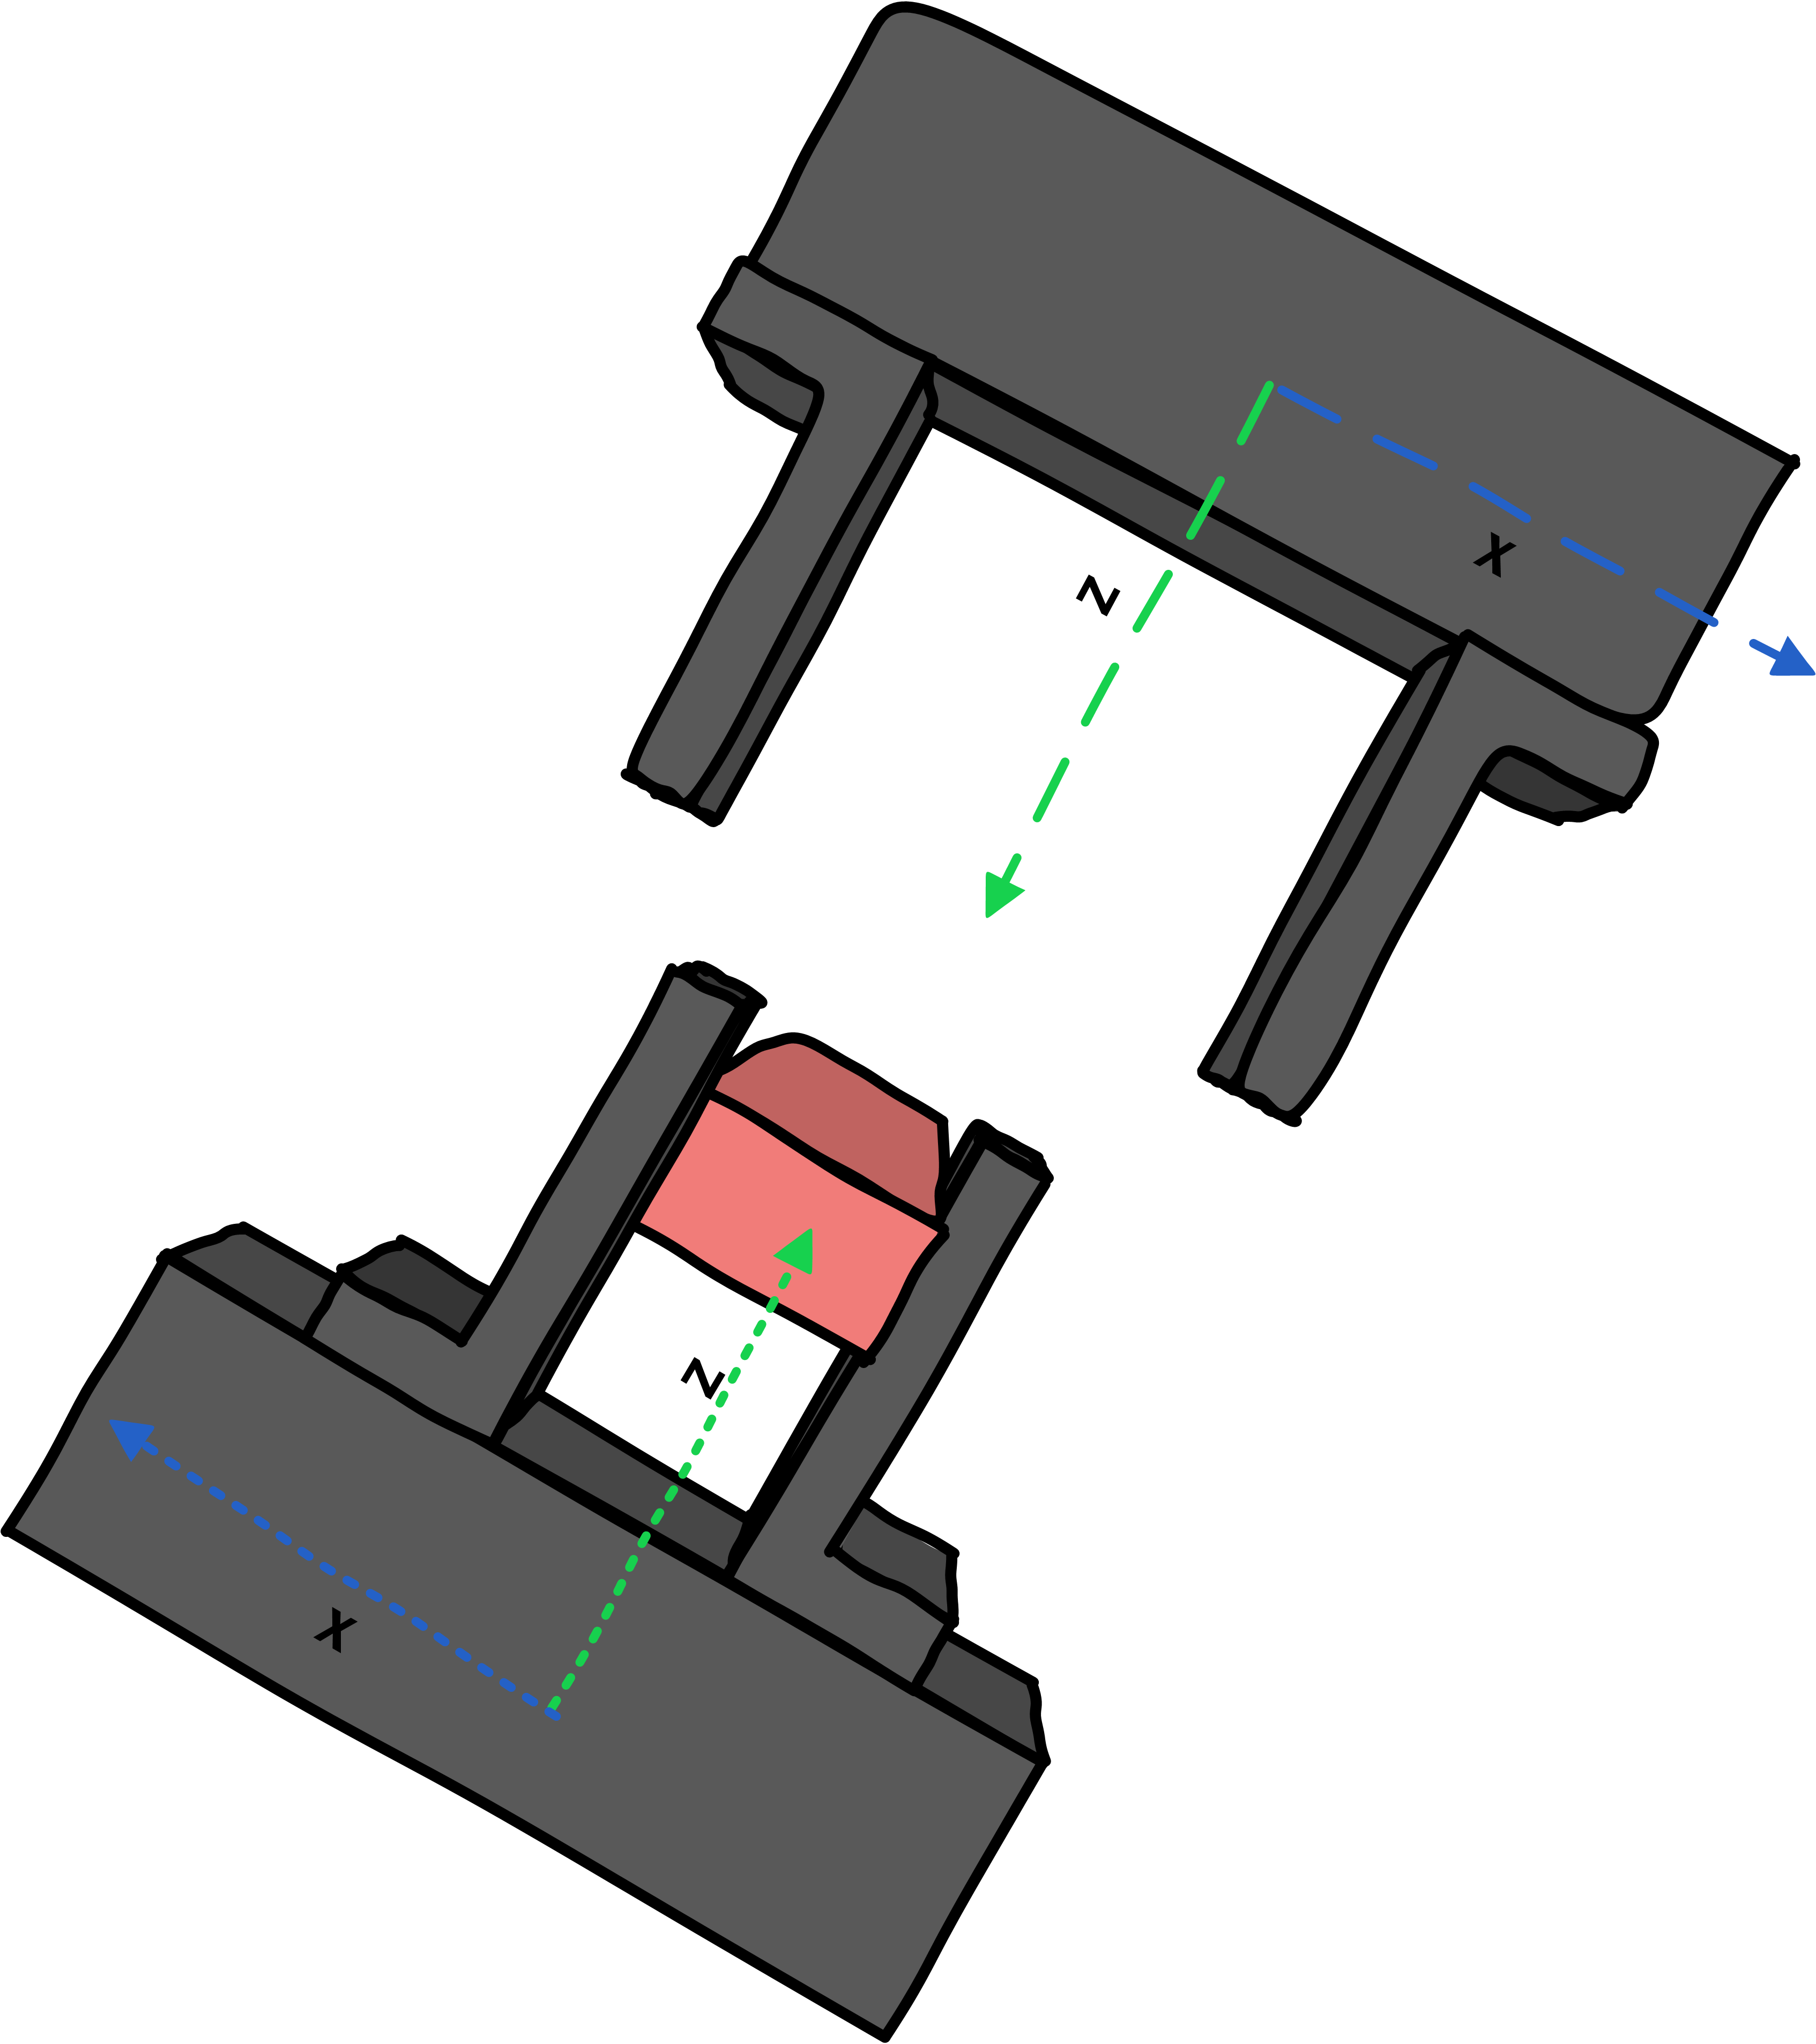
\includegraphics[scale=0.45]{fig/grip1}
 		\label{fig:grip1}}
 	\hfill
 	\subfigure[Translation($T_\tau$) an der X-Achse (blau) des Objektes (rose) zur Kollisionsvermeidung der Finger (grau). Die minimale Länge der Translation beträgt die Hälfter der aufsummierten Breite der Finger.]{%
 		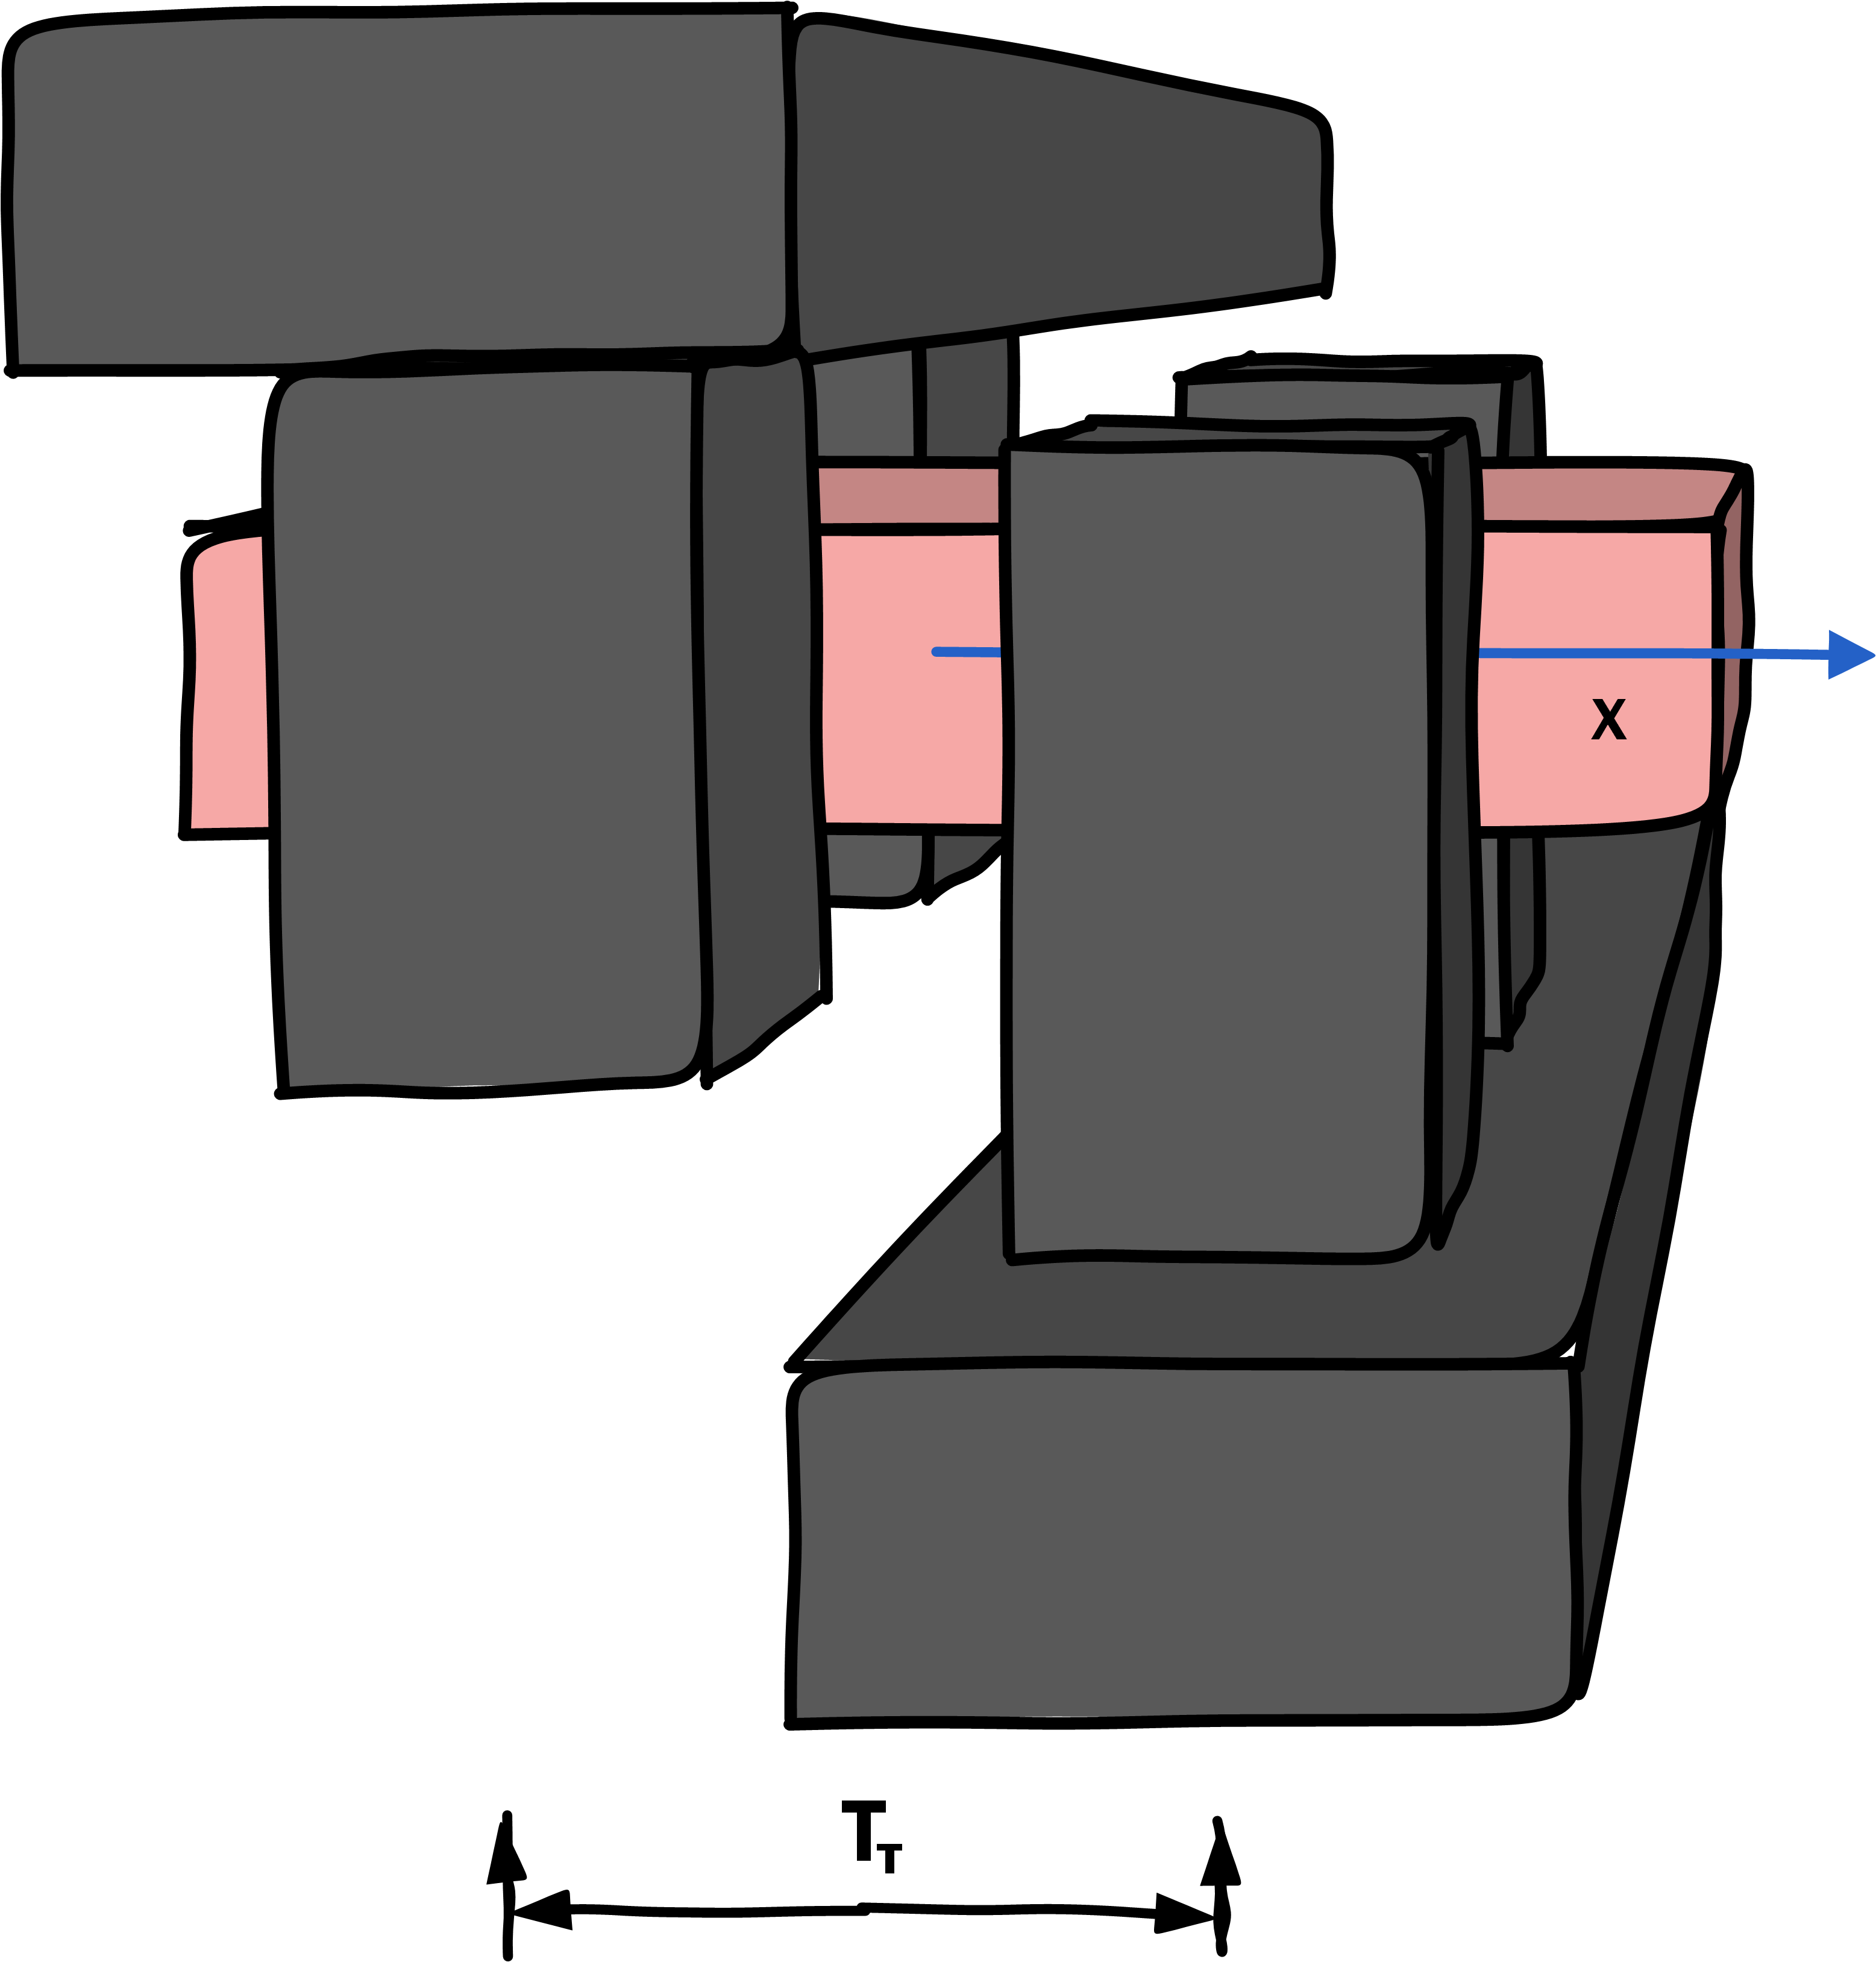
\includegraphics[scale=0.45]{fig/grip3}
 		\label{fig:grip3}}
 	
 	\caption{Greifer bei der Übergabe}
 	\label{fig:grip}
 \end{figure}

Da diese Funktionalität ein MR-Task ist, werden Nachrichten zwischen den Agenten ausgetauscht, um den Ablauf zu koordinieren. Dieser Nachrichtenaustausch wird in den folgenden Sequenz-Diagrammen dargestellt und analysiert. Dabei werden die drei Arten der Übergabe Geben (Abbildung \ref{fig:gripper1}), Nehmen (Abbildung \ref{fig:gripper2}) und Rendezvous (Abbildung \ref{fig:gripper3}) auf die Anzahl der Nachrichten $k$, sowie deren Komplexität, untersucht. Ein weiterer Aspekt ist das zeitliche Verhalten $t$ und der Unterschied im Ablauf der drei Varianten.

\begin{figure}
	\centering
	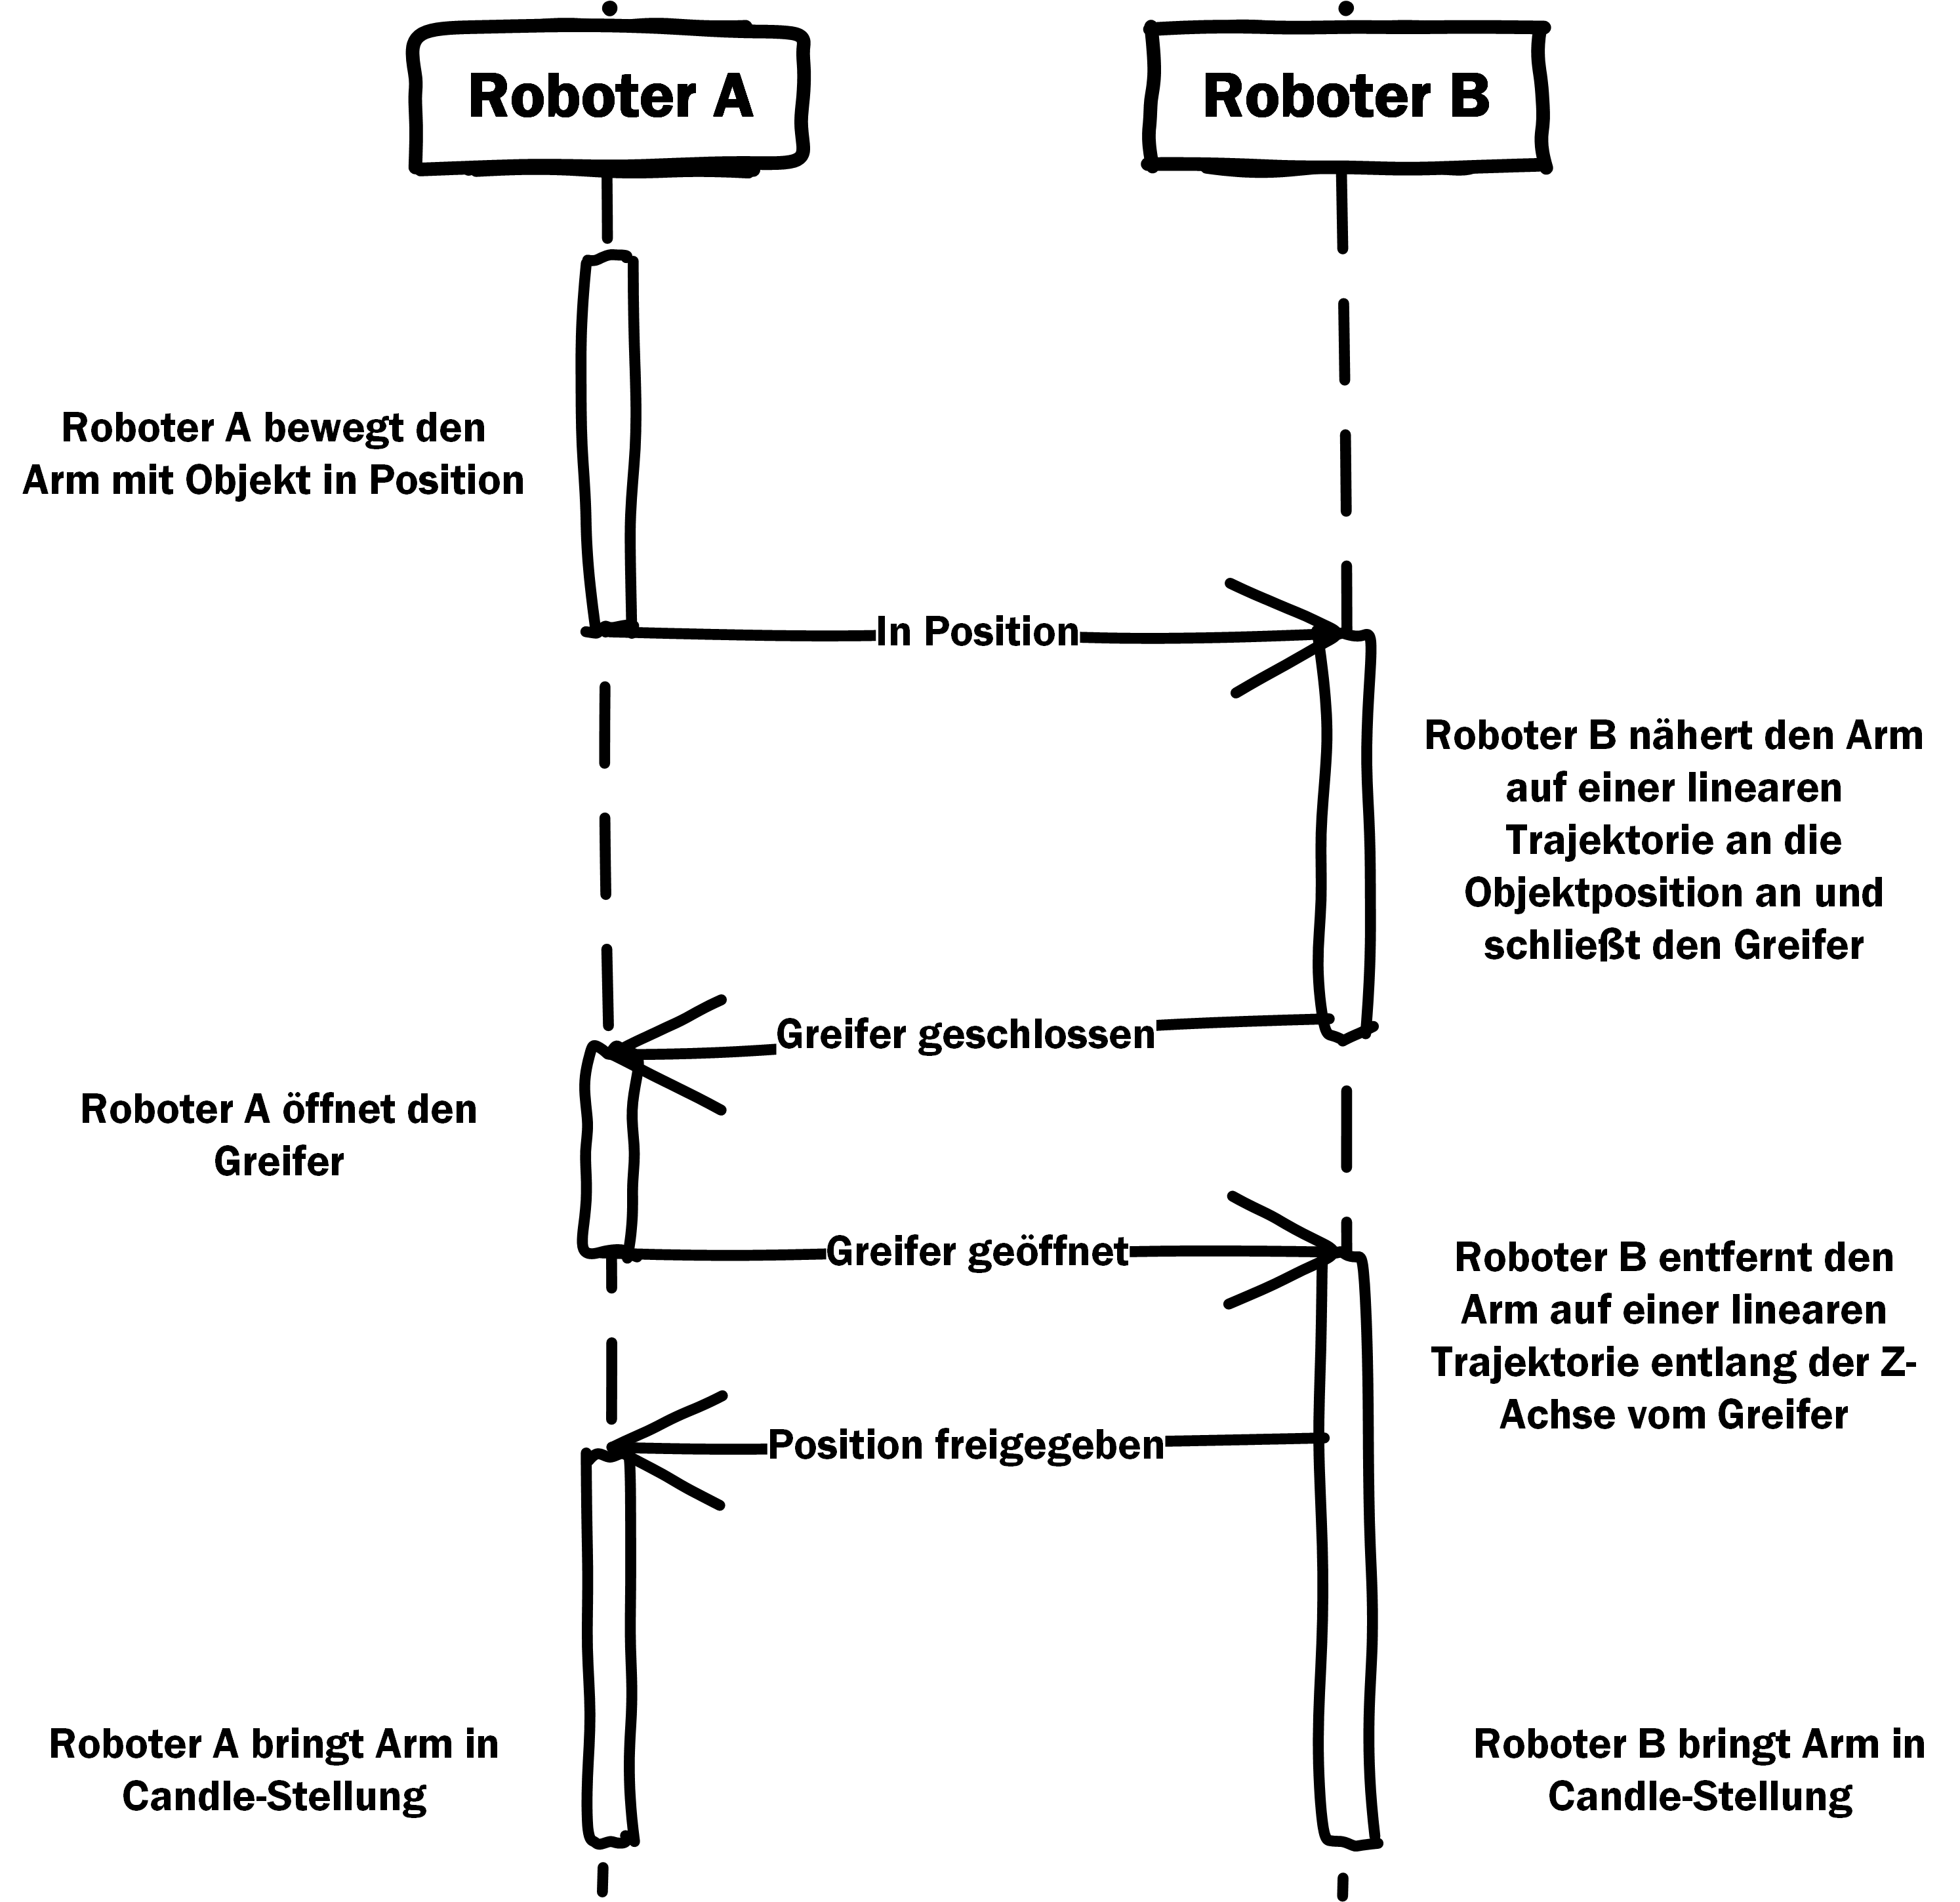
\includegraphics[scale=1.0]{fig/SeqGive}

	\caption[Sequenzdiagramm Geben]{Dieses Sequenzdiagramm zeigt den Ablauf des Gebens. Die Aktion wird dabei vom objekttragenden Roboter (A) initialisiert.}
		\label{fig:gripper1}
\end{figure}

Die in Abbildung \ref{fig:gripper1} dargestellte Variante des \textit{Gebens} wird von dem Roboter initialisiert, der das Objekt trägt (Roboter A). Nach Bestimmung der Übergabe Position und Orientierung bewegt sich zunächst Roboter A in die Pose. Dabei ist eine lineare Annäherung nicht nötig, da noch kein Kollisionspotential besteht. Anschließend wird eine einfache Bestätigung an Roboter B geschickt, der sich anschließend in Bewegung setzt. Diese besteht zunächst aus einer Positionierung nahe des Objektes. Der Greifer ist dabei schon geöffnet und dem anderen Greifer entgegengesetzt orientiert wie in Abbildung \ref{fig:grip1}. Folgend kommt die Annäherung auf der linearen Trajektorie entlang der Z-Achse an das Objekt. Sobald der Greifer in Position ist wird dieser geschlossen und eine einfache Bestätigung an den anderen Roboter gesendet. Dieser öffnet seinen Greifer und bestätigt ebenfalls. Durch diese Nachricht löst sich nun Roboter B, ebenfalls auf der Z-Achse, um das Objekt aus dem Greifer von Roboter A zu entfernen. Darauf folgt eine Freigabe an Roboter A, welcher sich nun auch von der Position entfernt, und der Übergang in die sichere Candle-Stellung.

Alle Nachrichten, die in dieser Variante ausgetauscht werden, sind einfache Bestätigungen oder Freigaben, die nur vom Zeitverhalten her dynamisch sind und keine weiteren Informationen beinhalten. Benötigt werden, ohne die Positionsbestimmung, vier Nachrichten zur vollständigen Koordinierung ($k_{Geben} = 4$). Für das Zeitverhalten gilt: $t_{Geben} = move_A + move_B + near_B + close_B + open_A + near_B + max(move_A, move_B)$ unter der Bedingung, dass $move_B \gg open_B$, da der Greifer von B während der Bewegung geöffnet wird. $move$ entspricht dabei der Zeit die für eine Bewegung von einer Pose in eine Zielpose benötigt wird, $near$ ist die Zeit für die positive oder negative Annäherung, $open$ und $close$ sind die benötigten Zeiten für das Öffnen und Schließen der Greifer.

\begin{figure}
		\centering
	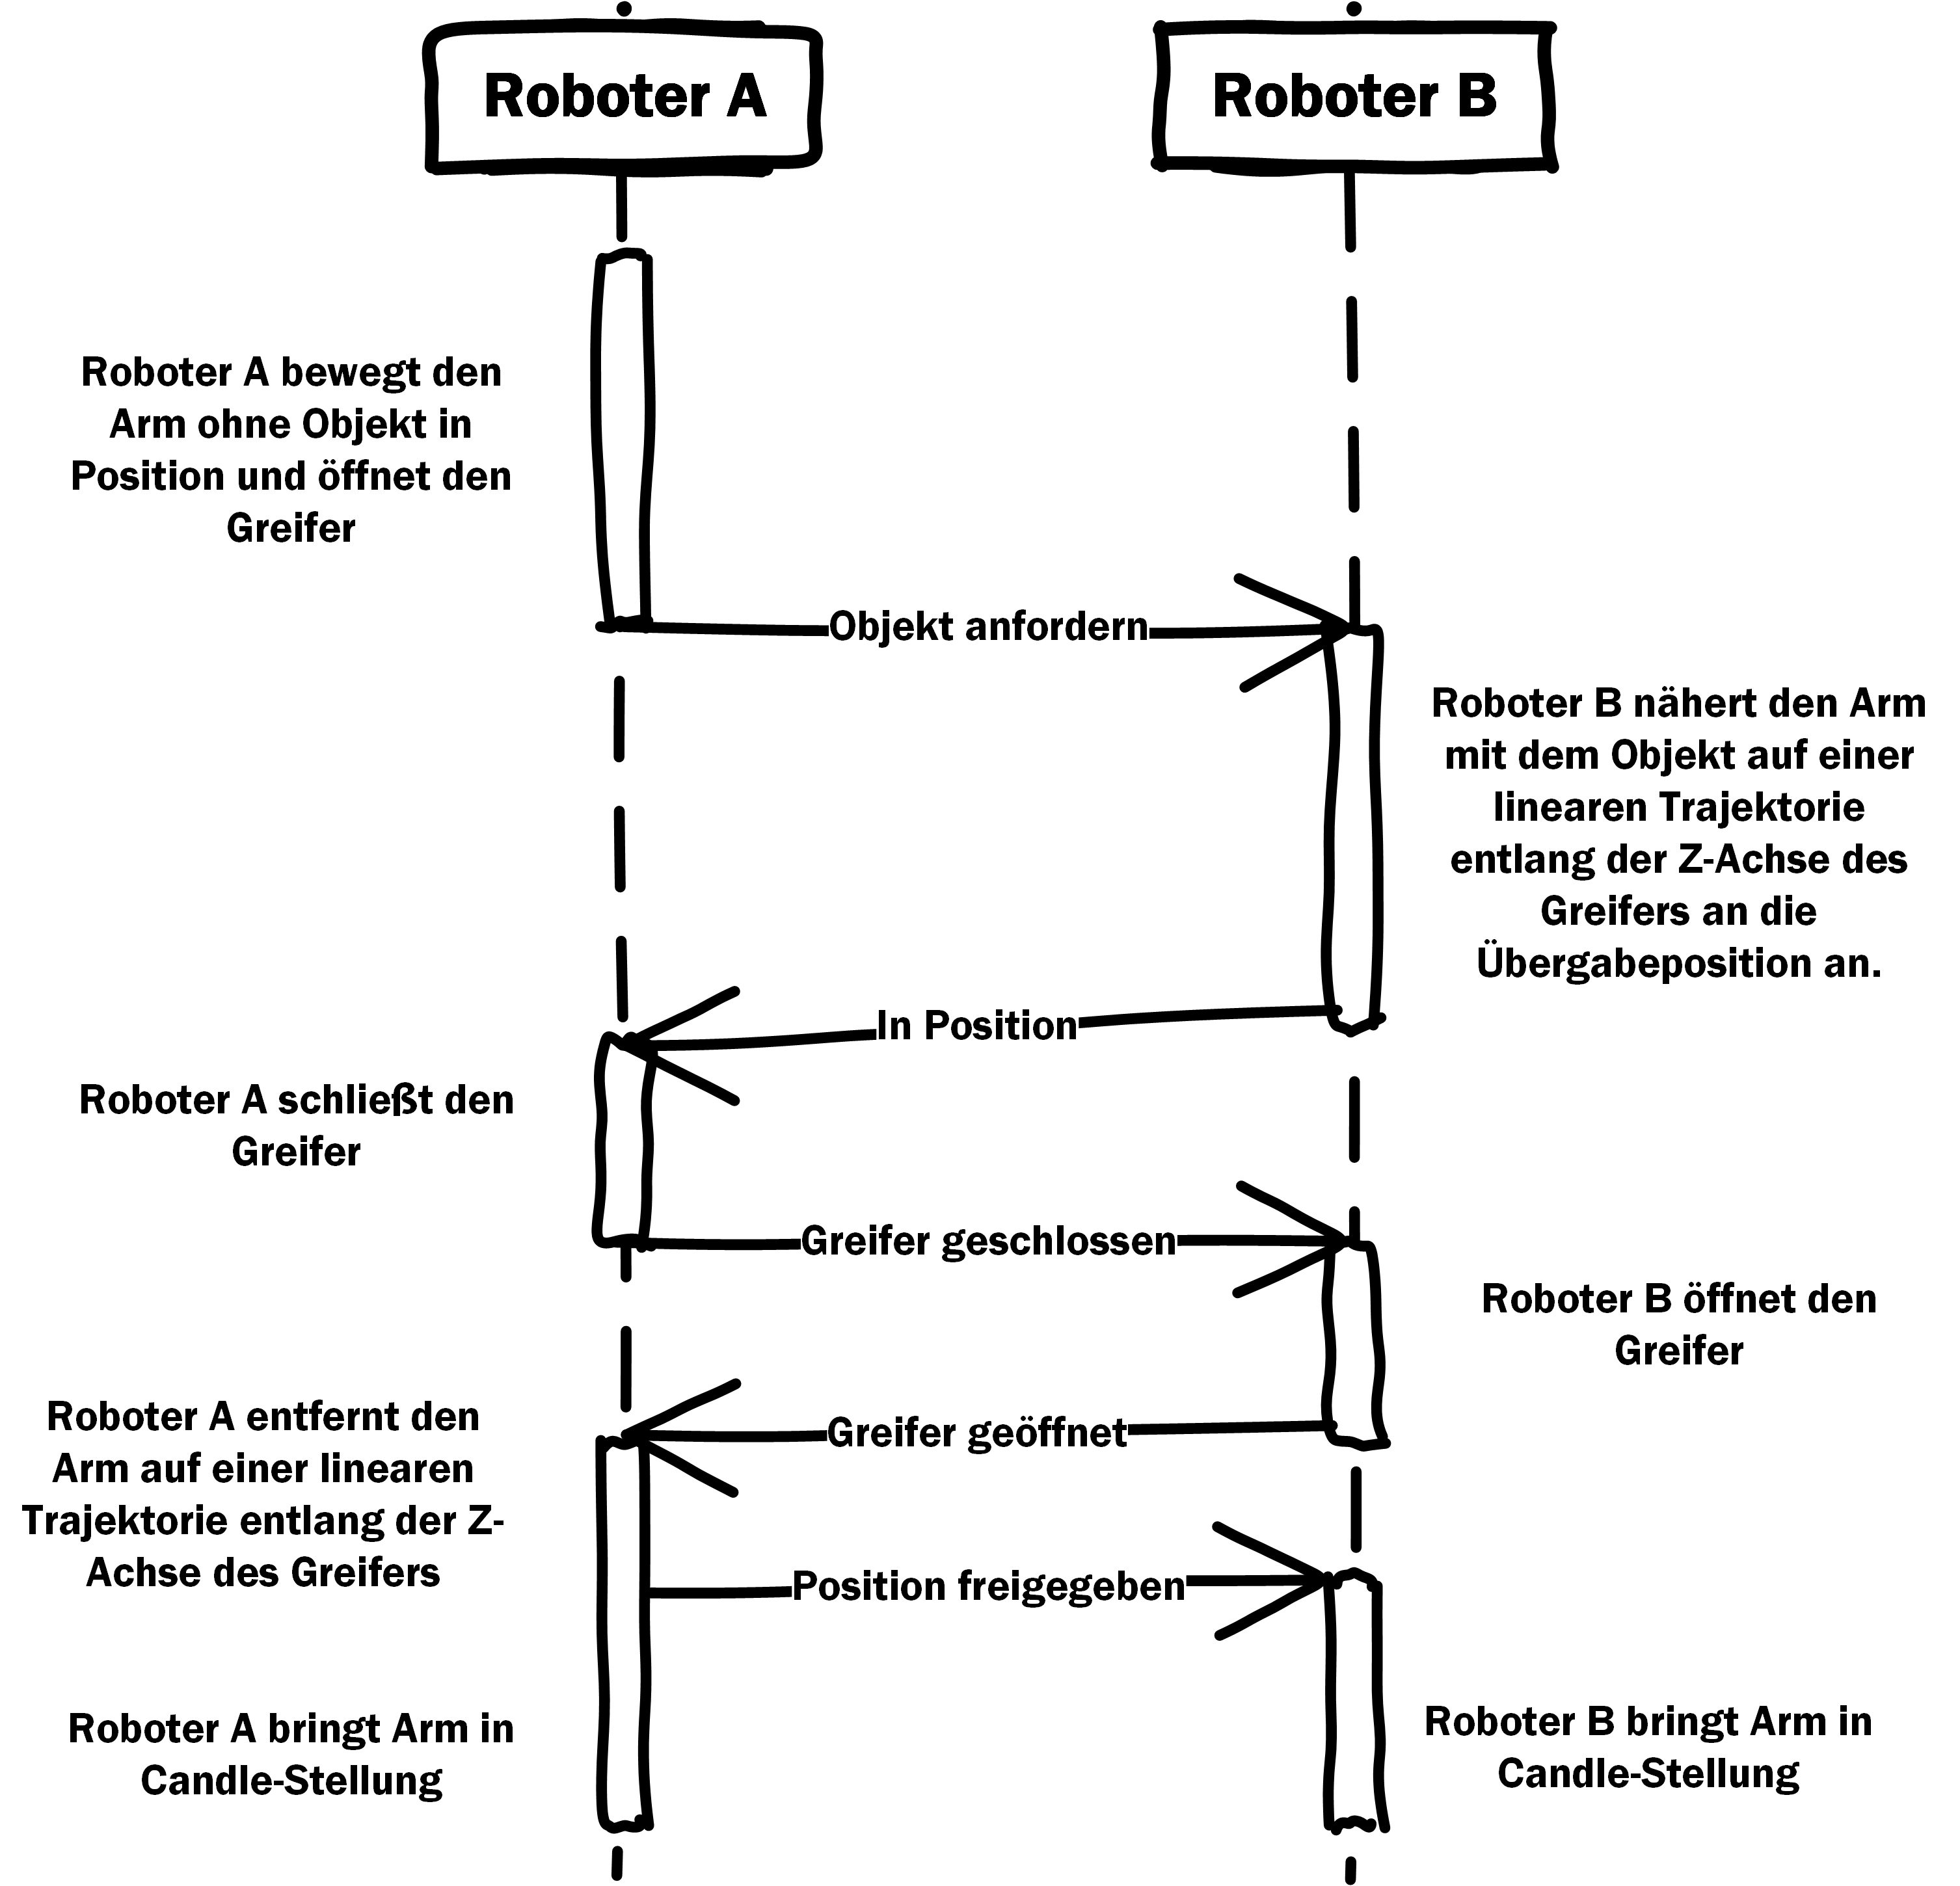
\includegraphics[scale=1.0]{fig/SeqTake}

\caption[Sequenzdiagramm Nehmen]{In diesem Sequenzdiagramm wird der Ablauf des Nehmens abgebildet. Die Aktion wird dabei vom objektlosen Roboter initialisiert.}
	\label{fig:gripper2}
\end{figure}

In Abbildung \ref{fig:gripper2} ist das \textit{Nehmen} dargestellt. Im Gegensatz zum \textit{Geben} wird die Aktion vom dem Roboter initialisiert, an den das Objekt übergeben wird. Nach der Positionsbestimmung bewegt Roboter A den Greifer ohne Objekt an die Übergabeposition und öffnet diesen während der Bewegung. Anschließend fordert er das Objekt an. Darauf nähert sich Roboter B mit dem Objekt auf der linearen Trajektorie entlang der Z-Achse dem Greifer A an und führt den Gegenstand zwischen den Fingern von Greifer A ein. Nach einer Positionsbestätigung schließt Roboter A den Greifer. In diesem Zustand wird das Objekt von beiden Robotern fixiert. Nach der Schließung des Greifers schickt Roboter A eine Nachricht an Roboter B, welcher nun seinen Greifer öffnet und dies mit einer Nachricht bestätigt. Roboter A entfernt nun das Objekt aus dem Greifer von Roboter B und gibt die Position frei nachdem er den Kollisionsraum verlassen hat. Anschließend bewegen beide Roboter die Arme in die sichere Candle-Stellung.

Der Nachrichtenaufwand dieser Variante beträgt $k_{Nehmen} = 5$. Wie beim \textit{Geben}, ist die Komplexität der Nachrichten eher gering, da es sich nur um zeitkritische Freigaben handelt. Für das Zeitverhalten gilt, unter den gleichen Bedingungen und Angaben wie beim \textit{Geben}: $t_{Nehmen} = move_A + move_B + near_B + close_A + open_B + near_A + max(move_A, move_B)$.


\begin{figure}
		\centering
	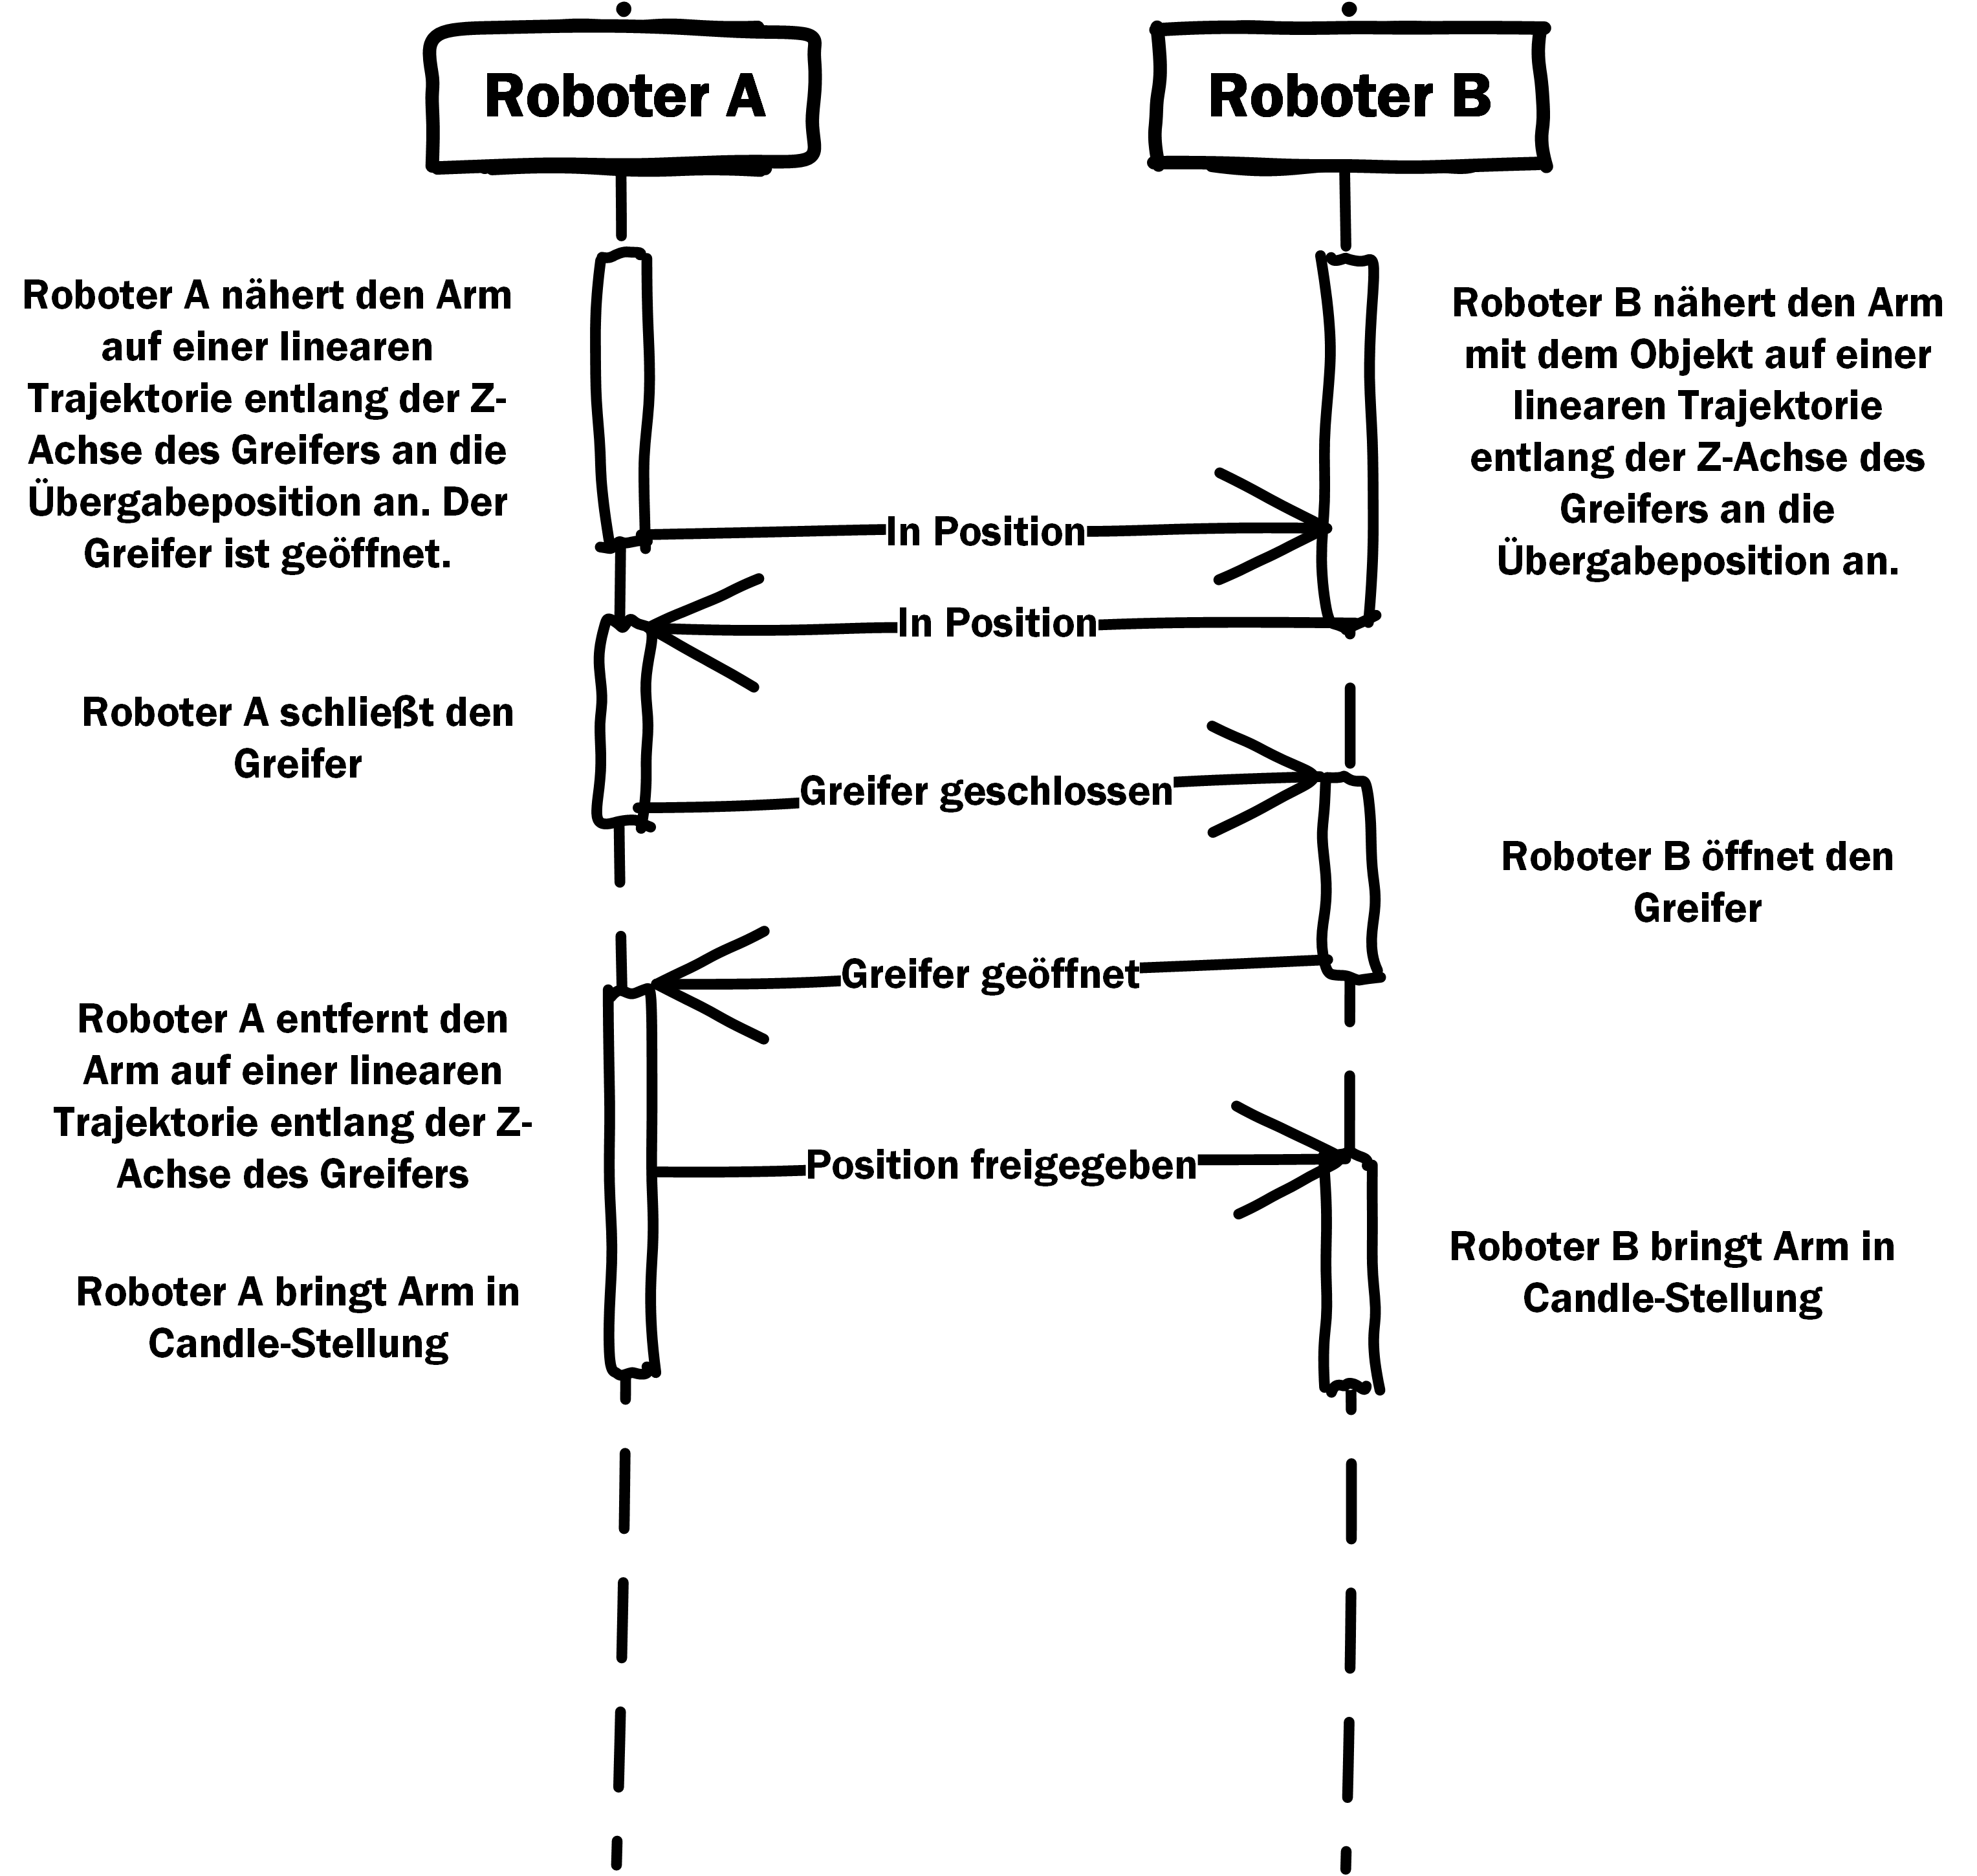
\includegraphics[scale=1.0]{fig/SeqRond}

\caption[Sequenzdiagramm Rendezvous]{Dieses Sequenzdiagramm zeigt die Rendezvous Variante der Übergabe. Die Aktion kann von beiden Agenten initialisiert.}
\label{fig:gripper3}
\end{figure}



Die Rendezvous-Übergabe in Abbildung \ref{fig:gripper3} wird die Initialisierungsbewegung nicht explizit von einem Roboter ausgeführt, sondern von beiden gleichzeitig. Dabei bewegen sich zunächst beide Arme auf die Übergabeposition, wobei sich beide Greifer das letzte Wegstück auf der linearen Trajektorie annähern. Beide Roboter bestätigen ihre Position, sobald sie diese erreicht haben. Anschließend schließt der Roboter A, ohne Objekt, den Greifer und bestätigt.Roboter B öffnet den Greifer und übergibt so das Objekt. Wie bei den anderen Varianten bewegt sich Roboter A nach einer Nachricht nun mit Objekt auf einer linearen Bahn von Greifer B weg. Nach der anschließenden Positionsfreigabe bewegen sich beide Roboter in die sichere Candle-Stellung.

Die Nachrichtenkomplexität ist bei dieser Variante etwas höher, als bei den anderen. Den Unterschied macht die erste Koordinierung, nachdem beide Arme in Position gegangen sind, da nicht definiert ist, welcher Roboter zuerst die Stellung erreicht und somit die Reihenfolge der Nachrichten nicht definiert ist. Die Komplexität des Inhaltes bleibt bei dieser Variante genauso gering, wie bei den anderen Variante, da es sich nur um Bestätigungen handelt. Die Anzahl der Nachrichten für diese Variante ist $k_{Rendezvous} = 5$. Für das Zeitverhalten gilt, unter den bekannten Bedingungen und Angaben:  $t_{Rendezvous} = max(move_A + near_A, move_B + near_B) + close_A + open_B + near_A + max(move_A, move_B)$.

Ein Vergleich der Kennzahlen der Varianten zeigt, dass der Koordinierungsaufwand beim \textit{Geben} am geringsten ist. Dies liegt vor allem an der Anzahl der Nachrichten: $k_{Geben} < k_{Nehmen} = k_{Rendezvous}$. Außerdem ist die Komplexität der Nachrichten untereinander identisch, mit der Ausnahme am Anfang der \textit{Rendezvous}-Variante. Für das Zeitverhalten gilt $t_{Rendezvous} < t_{Geben} = t_{Nehmen}$. Dies liegt vor allem an der Parallelisierung der Bewegung am Anfang der Aktion.


\paragraph{Einordnung}
Diese Funktion ist eng-gekoppelt und benötigt einen hohen Aufwand an Koordinierung. Neben der Übergabeposition und -orientierung müssen auch die Zeitvorgaben für das Öffnen und Schließen der Greifer, sowie die Bewegungen koordiniert werden. Dies macht diese Funktionalität zur komplexesten im ganzen System. Dies liegt vor allem daran, dass diese Funktion als MR-Task eingeordnet wird, da sie von zwei Agenten zusammen ausgeführt wird. Diese Agenten sollten Multi-Task fähig sein, da einige Subtasks parallel ausgeführt werden sollen, zum Beispiel das Öffnen des Greifers, während der Arm in eine Position fährt. Ebenfalls komplex ist die Positionsbestimmung der Übergabe. Zunächst müssen dabei die beiden Arbeitsräume einen Schnittraum aufweisen. Eine notwendige Positionskorrektur kann dabei nur vom mobilen Roboter ausgeführt werden. Dies muss unter anderem in der Konfiguration berücksichtigt werden. Dadurch steigt auch der Konfigurationsaufwand für die Aufgabe, da sichergestellt werden muss, dass die Arbeitsräume der beiden Roboter sich überhaupt schneiden können. Weitere Aspekte der Konfiguration sind die Kompatibilität der Greifer zum Objekt und die Erreichbarkeit der nachfolgenden Ziele.


\subsection{Agenten}
Aus den Nicht-Funktionalen Anforderungen und den Funktionen lassen sich die folgenden Agenten im MRS extrahieren. Diese Agenten bestehen aus den Sensoren aus Kapitel \ref{sec:aufbau-sensoren} und den Robotern Rose und Dummy. Für die Roboter steht die Zuweisung der Funktionen und Rollen im System fest, die anderen Aktoren und Sensoren werden den Funktionen zugewiesen. Für Funktionen bei denen unterschiedliche Sensoren oder Aktoren zur Verfügung stehen wird evaluiert welcher Hardware die Funktion am besten löst.

\subsubsection{Raumüberwachung}
Die Raumüberwachung ist zur Identifizierung und Lokalisierung von Objekten zuständig (siehe $f_2$\ref{sec:funraum}). Dabei soll das Kamerasystem eine große Fläche mit einer hohen Auflösung observieren. Als Hardware Lösungen standen dabei das XTion Kamera System oder der Argos3D Sensor zur Auswahl. Da der Tiefensensor jedoch eine kleinere Auflösung als die XTion hat und kein Farbbild liefert, wird für die Umsetzung des MRS die XTion ausgewählt. Diese wurde plangemäß nach Abbildung \ref{fig:basic-aufbau-teststand} und \ref{fig:basic-aufbau-teststandh} an der Wand montiert. Zur Befestigung wurde eine zusätzliche Halterung mit dem 3D-Drucker gedruckt. Diese ermöglicht einen größeren Winkel in der Ausrichtung. Der eingestellte Winkel beträgt -62 \textdegree um die globale X-Achse. Durch die Höhe und den eingestellten Winkel ergibt sich eine Observerationsfläche auf der globalen X-Y-Ebene von 5,075 $m^2$. In Abbildung \ref{fig:imghawk} sieht man eine aufgenommene Punktwolke der angebrachten Kamera. Auf dieser ist die Trapezform der Punktwolke sehr gut sichtbar. Diese ergibt sich aus der Position und Orientierung der Kamera. Bedingt dadurch weisen nähere Objekte eine größere Punktdichte auf als entfernte Objekte. Auf der Abbildung sind zwei Bereiche ohne Punkte markiert. Die blaue Markierung zeigt auf eine Verschattung durch den Roboterarm. Der grüne Bereich weist viele schlecht gematchte Punkte zwischen Farb- und IR-Bild auf. Dies liegt vor allem an den schlecht reflektierten IR-Punkten auf dem Heizkörpergitter.

\begin{figure}
	\centering
	\includegraphics[scale=1.0]{fig/imghawk}
	\caption[Raumüberwachung Aufnahme]{Aufnahme der XTion als Raumüberwachung. Blaue Markierung: Toter Winkel der IR Aufnahme. Grüner Markierung: Heizkörper mit diffusen IR-Reflektionen.}
	\label{fig:imghawk}
\end{figure}

\subsubsection{Nahfelderkennung}
Die Nahfelderkennung setzt die Funktionalität $f_3$ (siehe \ref{sec:funnah}) um. Dabei wird der Sensor auf dem mobilen Roboter befestigt, um ein Objekt auch im Nahfeld identifizieren und lokalisieren zu können. Die Lokalisierung soll dabei wesentlich genau sein, als bei der Raumüberwachung. Zur Auswahl standen dabei wieder die XTion und der Argos3D Sensor. Der Vorteil des Sensors ist die geringe minimale Reichweite. Diese funktioniert schon ab 100 mm, während die XTion einen mindest Abstand von 800 mm braucht. So ist eine Montage des Argos Sensors am Greifer direkt möglich, während die XTion mit Abstand montiert werden muss. Nachteil ist die zusätzliche Stromversorgung, die der Sensor benötigt, und der fehlende Farbkanal. Dennoch wurde der erste Prototyp mit dem Argos3D Sensor entwickelt.

\subsubsection{Lokalisierung}



\subsection{Architektur RATS}
\subsection{Inverse Kinematik}

